% ============================================================================
% Chapter 5 — Performance Evaluation and Analysis
% Rubric-mandated six-section top level (5.1 to 5.6) plus the signpost.
% Course outcomes covered: CO6 (analyse alternatives, performance), CO7
% (final design adjustments). Section titles are fixed by the rubric.
% ============================================================================

\chapter{Performance Evaluation and Analysis}
\label{ch:evaluation}

% Chapter scope: Section 5.1 reports the results of the main run; 5.2 the
% cycle-zero choices that fixed the configuration; 5.3 the statistical
% tests; 5.4 the comparison with external baselines and the classifier
% ablation; 5.5 the summary and hypothesis verdicts; 5.6 the discussion.

\section{Performance Evaluation}
\label{sec:performance}

\subsection{Experimental setup}
\label{sec:setup}

\subsubsection{Benchmarks and the training-versus-transfer split}
\label{sec:setup-benchmarks}

Five benchmarks are used. The \textbf{training panel} is FEVER \cite{thorne-etal-2018-fever} (claim verification), TriviaQA \cite{joshi-etal-2017-triviaqa} (open-domain trivia) and CommonsenseQA \cite{talmor-etal-2019-commonsenseqa} (five-option commonsense questions). The \textbf{transfer panel} is TruthfulQA \cite{lin-etal-2022-truthfulqa} (common misconceptions) and StrategyQA \cite{10.1162/tacl_a_00370} (implicit multi-step yes-or-no questions). Only the training panel feeds the calibration fold, the seed pool, the stream chunks and the training pool; the transfer panel is evaluated only, to measure how the system behaves on questions unlike those it learns from. The retention guard uses three separate probes: MMLU \cite{hendrycks2021measuring} and held-out test slices of TriviaQA and CommonsenseQA. HotpotQA and Natural Questions were dropped before the main run because the base generator answered too few of their questions correctly ($0.09$ and $0.17$) for the gate to build a usable pool (\Cref{sec:scope-research}).

Each training benchmark is split into six disjoint folds (\Cref{tab:benchmark-pools}): a seed pool for the cold-start memory, a calibration fold, a purity-validation slice, ten stream chunks (one per possible cycle), an evaluation fold of $300$ questions used for every headline number, and a test fold kept for later work. The transfer benchmarks have only evaluation and test folds. All folds were checked for overlap by content hash when they were built.

\begin{table}[!htbp]
\centering
\small
\begin{tabular}{@{}p{2.6cm}p{1.5cm}p{1.0cm}p{1.0cm}p{1.0cm}p{2.0cm}p{1.0cm}p{1.0cm}@{}}
\toprule
\textbf{Benchmark} & \textbf{Panel} & \textbf{Seed} & \textbf{Calib} & \textbf{Purity} & \textbf{Stream chunks} & \textbf{Eval} & \textbf{Test} \\
\midrule
FEVER             & training & $1000$ & $500$ & $500$ & $10\times 2000$ & $300$ & $500$ \\
TriviaQA          & training & $1000$ & $500$ & $500$ & $10\times 2000$ & $300$ & $500$ \\
CommonsenseQA     & training & $1000$ & $500$ & $500$ & $10\times 700$  & $300$ & $500$ \\
TruthfulQA        & transfer & $0$    & $0$   & $0$   & $0$             & $300$ & $500$ \\
StrategyQA        & transfer & $0$    & $0$   & $0$   & $0$             & $300$ & $387$ \\
\bottomrule
\end{tabular}
\caption[Benchmark folds.]{Benchmark folds. CommonsenseQA has smaller stream chunks because its training split holds only about $10{,}000$ questions after de-duplication; the StrategyQA test fold is limited by the size of its split.}
\label{tab:benchmark-pools}
\end{table}

\subsubsection{Metrics}
\label{sec:setup-metrics}

\textbf{Exact match (EM):} the main accuracy measure, read from the final answer line of each response by one rule for every system. FEVER and StrategyQA are scored by the label the answer starts with; CommonsenseQA by the single option letter given, where the option text may follow the letter but two letters count as wrong; TriviaQA by exact match against any gold alias after normalisation. TruthfulQA is scored by a language-model judge (Claude Haiku) that compares the final answer with the benchmark's correct and incorrect reference answers, following the judge-based evaluation introduced with the benchmark \cite{lin-etal-2022-truthfulqa}; a refusal counts as correct only when the reference answers include one. The same judge, reading the same part of the response, scores every system.

\textbf{Composite hallucination metric (CHM):} the equal-weighted mean of seven failure rates, each computed over all evaluation questions.
\begin{itemize}
    \item \textbf{Confident confabulation:} the answer is wrong but its stored score $\ustored$ is at least $0.50$.
    \item \textbf{Factual fabrication:} the answer is wrong and its weakest atomic fact has passage support below $0.30$.
    \item \textbf{Logical fabrication:} the answer is wrong and the model's own chains support it below $0.30$.
    \item \textbf{Defensive evasion:} the answer is wrong and uses an evasive phrase such as \emph{the context does not mention}.
    \item \textbf{Template leakage:} the output contains a leaked prompt placeholder.
    \item \textbf{False refusal:} the answer is correct but the system abstained or discarded it.
    \item \textbf{Over-long output:} the answer is wrong and longer than $600$ characters.
\end{itemize}
Two of these, confident confabulation and false refusal, are defined through the system's own verifier, so they move with the gate's operating point: a more permissive gate refuses fewer correct answers and lets more wrong answers keep a high score. Two further rates are recorded but left out of the mean, because neither can fire in this run:
\begin{itemize}
    \item \textbf{Factual contradiction:} the entailment judge returns only a support probability, with no contradiction output.
    \item \textbf{Off-topic:} planned as a wrong answer whose question-match score is below $0.50$. That score cannot detect off-topic answers on this panel, and its stored values never fall below $0.50$ (\Cref{sec:verifier-qa-rel}). An attempt after the run to measure off-topic answers directly, with a language-model judge, was checked against $200$ hand-labelled answers and agreed too weakly to give a reliable rate (Cohen's kappa about $0.35$), so measuring them is left to future work.
\end{itemize}

\textbf{Model view and delivered view:} every system is reported in two views. The \emph{model view} scores EM and CHM on every raw answer the generator wrote, including answers that CAEM then withheld; it measures what the model knows. The \emph{delivered view} scores what the user receives. CAEM shows every answer with its probability and a status tag (verified, provisional or conflicting, \Cref{sec:decision}) except abstentions, which hide the answer behind an insufficient-evidence message; semantic-entropy abstention (B8) withholds the answers it abstains on; every other baseline answers every question. Following the selective-prediction setting of Kamath et al.~\cite{kamath2020selective} and Geifman and El-Yaniv~\cite{geifman2017selective}, the delivered view reports the share of questions answered, the share of those answers that are wrong, and CHM over the answered questions; for CAEM it also reports the accuracy of each status tag, because the tag is part of what the user sees. Unlike the two verifier-defined rates, the answered share and the error among answered do not depend on the verifier's scores.

\textbf{Composite evaluation score (CES):} a single summary of five axes, each in $[0,1]$ with one best: accuracy (pooled EM), epistemic quality ($1 - \mathrm{CHM}$), retention (worst probe ratio, capped at one), calibration ($1 - 2\,\mathrm{ECE}$) and verifier reliability ($\max(2\,\mathrm{BA} - 1, 0)$, with the balanced accuracy approximated as $\Phi(d/\sqrt{2})$ from the calibration-fold Cohen's $d$). The score is the geometric mean, so a collapse on one axis is not averaged away:
\begin{equation}
\mathrm{CES} = \left(\prod_{i=1}^{5} \mathrm{clamp}_{[\varepsilon,1]}(\mathrm{axis}_i)\right)^{1/5}, \quad \varepsilon = 0.01.
\label{eq:ces}
\end{equation}

\textbf{Retention ratio:} accuracy on each probe divided by its value before any fine-tuning (\Cref{eq:nfr-retention-floor}); the worst probe decides whether a cycle is kept. \Cref{tab:metrics} summarises the metrics.

\begin{table}[!htbp]
\centering
\small
\begin{tabular}{@{}>{\raggedright\arraybackslash}p{3.8cm}>{\raggedright\arraybackslash}p{3.4cm}>{\raggedright\arraybackslash}p{7.0cm}@{}}
\toprule
\textbf{Metric} & \textbf{Reported on} & \textbf{Definition} \\
\midrule
Exact match (EM) & all five benchmarks & label or alias match; TruthfulQA judged by Claude Haiku against the reference answers \\
Composite hallucination metric (CHM) & all five benchmarks & mean of seven failure rates \\
Answered, wrong among answered & pooled & delivered view: share not withheld; share of those that are wrong \\
Status-tag accuracy & pooled, CAEM & share of questions and EM per tag shown to the user \\
Storage precision $\pi_{\text{store}}$ & per cycle & share of stored answers that are correct \\
Gate balanced accuracy, Cohen's $d$ & calibration fold & $(\mathrm{TPR} + 1 - \mathrm{FPR})/2$ at $\tau_{\text{store}}$; separation of correct and incorrect scores \\
Composite evaluation score (CES) & pooled & geometric mean of five axes (\Cref{eq:ces}) \\
Retention ratio & probe panel & worst probe accuracy over its pre-fine-tuning value \\
\bottomrule
\end{tabular}
\caption[Metrics reported in this chapter.]{Metrics reported in this chapter.}
\label{tab:metrics}
\end{table}

\subsubsection{Comparison protocol}
\label{sec:setup-protocol}

The external baselines (\Cref{sec:external-baselines}) are compared with CAEM under one protocol, so that a difference in the results reflects the method rather than the prompt or the scoring.
\begin{itemize}
    \item \textbf{Matched prompts:} every baseline that answers from the question alone receives CAEM's zero-shot question message: the same system instruction, worked example, task line, answer format and forced reasoning prefix. Chain of thought (B2) and five-shot chain of thought (B5) add the step-by-step cue to that message; B5's five demonstrations per benchmark are drawn from the benchmark's training split (for TruthfulQA, which has a single split, from the questions not evaluated), with every evaluated question removed. The two retrieval baselines (B3, B4) use CAEM's retrieval prompt with the same top five passages, vanilla fine-tuning (B6) is evaluated with the prompt it was trained on, which is CAEM's zero-shot message, and FLARE (B7) uses the zero-shot message for its draft and its final answer.
    \item \textbf{One scoring rule:} every system is scored by the rules of \Cref{sec:setup-metrics}, applied to its final answer line, and every TruthfulQA answer by the same judge.
    \item \textbf{One hallucination instrument:} CHM needs verifier signals, so each baseline answer is passed through CAEM's verifier with the adapter and composite of cycle three, the same instrument for every baseline. The decision the verifier would take on a baseline answer is only a measurement: the baseline never acted on it. A baseline is therefore never charged with a false refusal or a withheld answer from CAEM's decision rule; its withheld answers are only those it withheld itself (B8).
    \item \textbf{Same questions:} every system answers the same $1{,}500$ evaluation questions, in the same order, checked question by question before scoring.
\end{itemize}
CAEM's outputs come from the main run. An earlier comparison had given the baselines a shorter prompt than CAEM's and scored some answer formats differently, so after the main run the baselines were re-run under this protocol (B3 and B4 only on TruthfulQA, where a graphics-memory error had left the first batch of $32$ questions unanswered; their prompts were already CAEM's). CAEM's own prompts are identical, character for character, in the code of the main run and of the re-run.

\subsubsection{Hardware, seed, reproducibility}
\label{sec:setup-reproducibility}

All phases ran on one rented graphics processor of the $32$-gigabyte class, under a single recorded random seed. The main run took cycles zero to five and stopped after cycle five as planned after the cycle-four rollback (\Cref{sec:env-cycles}). The baseline re-run of \Cref{sec:setup-protocol} used a second machine of the same class. For that re-run, the passages for the evaluation questions were retrieved once by exact search over the same index and reused; on a check sample, live search returned the same passages for $50$ of $50$ questions, and the verifier's passage scores from the main run were reproduced within $0.01$ on $98$ percent of answers. Signals computed from sampled text (dropout agreement, chain similarity and chain entailment) are random draws by design and differ slightly between runs. The code, the configuration files and the per-cycle artefacts are listed in \Cref{app:reproducibility}.

\subsection{Trajectory of headline metrics}
\label{sec:headline-trajectory}

All results in this section use the locked configuration chosen at cycle zero; \Cref{sec:final-adjustments} explains how it was chosen. The section order follows the BRAC template rather than the order in which the work was done.

\subsubsection{The headline in three steps}
\label{sec:headline-pooled}

\Cref{tab:headline-steps} separates the three contributions that a single before-and-after comparison would mix together: the architecture (B1, the same generator answering zero-shot with the same prompt, to C0, CAEM before any fine-tuning), the self-improvement loop (C0 to C5) and the whole system (B1 to C5). Significance is read from the paired per-benchmark tests of \Cref{sec:comp-baselines}.

% Auto-generated by scripts/build_ch5_evidence_tables.py; EM/CHM/subtypes from outputs/analysis/chm_judged.json
% (Haiku-judged TruthfulQA); coverage and error-among-answered from the
% per-sample evaluation files (ABSTAIN = not answered; TruthfulQA uses the judged correctness field).
\begin{table}[!htbp]
\centering\small
\setlength{\tabcolsep}{5pt}
\begin{tabular}{@{}lrrrrrr@{}}
\toprule
\textbf{System} & \textbf{EM} & \textbf{CHM} & \twoline{Confident\\confab.} & \twoline{False\\refusal} & \textbf{Answered} & \twoline{Wrong among\\answered} \\
\midrule
B1 (zero-shot) & $0.507$ & $0.137$ & $0.327$ & $0.055$ & $100.0\%$ & $0.493$ \\
CAEM C0 & $0.541$ & $0.134$ & $0.088$ & $0.298$ & $66.1\%$ & $0.381$ \\
CAEM C2 & $0.544$ & $0.110$ & $0.259$ & $0.057$ & $87.7\%$ & $0.425$ \\
CAEM C5 & $0.517$ & $0.117$ & $0.307$ & $0.065$ & $83.0\%$ & $0.451$ \\
\bottomrule
\end{tabular}
\caption[The headline in three steps.]{The headline in three steps on the five-benchmark evaluation fold ($1{,}500$ questions). B1 to C0 isolates the architecture, C0 to C5 the self-improvement loop, B1 to C5 the whole system.}
\label{tab:headline-steps}
\end{table}


% Auto-generated by scripts/build_ch5_evidence_tables.py from outputs/analysis/chm_judged.json (2026-10-19).
\begin{figure}[!htbp]
\centering
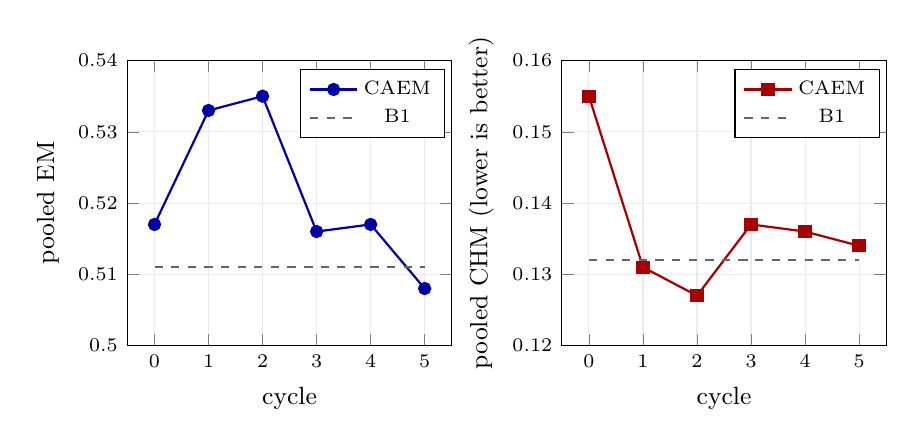
\begin{tikzpicture}
\begin{axis}[name=em, width=0.47\textwidth, height=5.2cm, xlabel={cycle}, ylabel={pooled EM}, xtick={0,...,5},
  ymin=0.50, ymax=0.54, font=\small, tick label style={font=\scriptsize}, grid=major, grid style={black!8},
  legend style={font=\scriptsize, at={(0.98,0.97)}, anchor=north east}]
  \addplot[blue!65!black, mark=*, thick] coordinates {(0,0.517) (1,0.533) (2,0.535) (3,0.516) (4,0.517) (5,0.508)};
  \addlegendentry{CAEM}
  \addplot[black!60, dashed, thick, domain=0:5] {0.511};
  \addlegendentry{B1}
\end{axis}
\begin{axis}[at={(em.east)}, anchor=west, xshift=1.4cm, width=0.47\textwidth, height=5.2cm, xlabel={cycle},
  ylabel={pooled CHM (lower is better)}, xtick={0,...,5}, ymin=0.12, ymax=0.16, font=\small,
  tick label style={font=\scriptsize}, grid=major, grid style={black!8},
  legend style={font=\scriptsize, at={(0.98,0.97)}, anchor=north east}]
  \addplot[red!65!black, mark=square*, thick] coordinates {(0,0.155) (1,0.131) (2,0.127) (3,0.137) (4,0.136) (5,0.134)};
  \addlegendentry{CAEM}
  \addplot[black!60, dashed, thick, domain=0:5] {0.132};
  \addlegendentry{B1}
\end{axis}
\end{tikzpicture}
\caption[EM and CHM by cycle against B1.]{Pooled EM (left) and CHM (right) by cycle on the evaluation fold, against B1. EM is level with B1 at C0, peaks at C2 and returns to B1's level by C5; CHM is above B1 at C0, where the system refuses too often, about level with it from C1, and ends just above it.}
\label{fig:trajectory}
\end{figure}


\textbf{The architecture adds almost no accuracy:} memory, routing, the retrieval-utility classifier and the verifier together move pooled EM from $0.511$ to $0.517$ before any fine-tuning (\Cref{fig:trajectory}), and from $0.554$ to $0.569$ on the training panel. No benchmark shows a significant EM difference between B1 and C0.

\textbf{The architecture alone is over-cautious:} at C0 the system abstains on $33.9$ percent of evaluation questions and discards another $31.9$ percent. False refusal reaches $0.276$, which lifts CHM to $0.155$, above B1's $0.132$, even though confident confabulation falls from $0.208$ to $0.089$. C0's CHM is significantly higher than B1's on TriviaQA, TruthfulQA and StrategyQA.

\textbf{Self-improvement helps for two cycles, then erodes:} after the first cycle the system abstains on $14.4$ percent and discards $9.7$ percent, false refusal falls to $0.059$ and CHM to $0.131$; EM rises to $0.533$ at C1 and $0.535$ at C2, the best values of the run. From C3 the gains fade: pooled EM ends at $0.508$ and CHM at $0.134$. On the training panel EM peaks at C1 ($0.584$, \Cref{tab:per-bench-trajectory}) and ends at $0.549$, below B1's $0.554$.

\textbf{Confident confabulation returns:} as the refitted gate becomes more permissive, confident confabulation rises to $0.259$ at C2 and $0.305$ at C5, above B1's $0.208$: after self-improvement, the verifier gives a high score to more of the generator's wrong answers than it gave to the base generator's. Because this rate and false refusal are both defined through the verifier's own score, they trade off: their sum is $0.365$ at C0, between $0.297$ and $0.329$ at C1 to C4 and $0.361$ at C5 (\Cref{fig:tradeoff}). The net CHM change from C0 to C5 ($0.155$ to $0.134$) comes from the other subtypes: fewer wrong answers with unsupported facts ($0.381$ to $0.327$), unsupported reasoning ($0.298$ to $0.245$) or evasive phrasing ($0.044$ to $0.003$).

% Auto-generated by scripts/build_ch5_evidence_tables.py (final drafting pass, 2026-10).
\begin{figure}[!htbp]
\centering
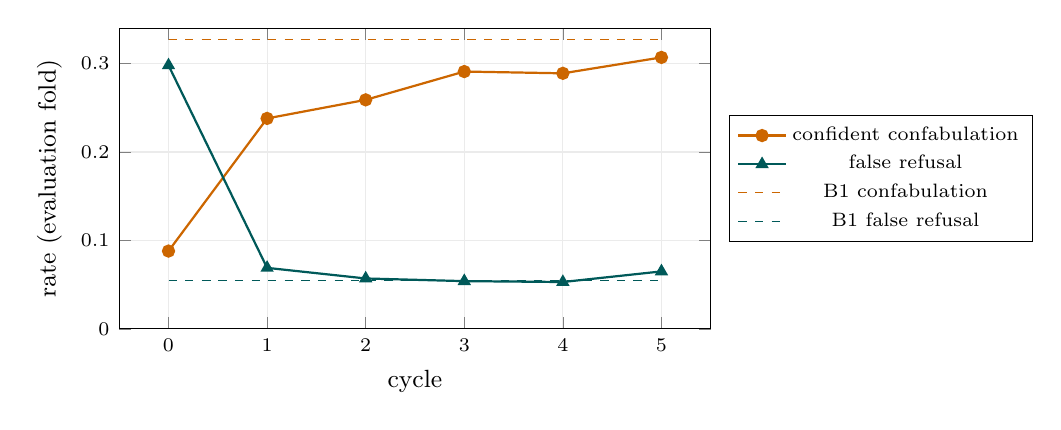
\begin{tikzpicture}
\begin{axis}[width=0.75\textwidth, height=5.4cm, xlabel={cycle}, ylabel={rate (evaluation fold)}, xtick={0,...,5},
  ymin=0, ymax=0.34, font=\small, tick label style={font=\scriptsize}, grid=major, grid style={black!8},
  legend style={font=\scriptsize, at={(1.03,0.5)}, anchor=west}]
  \addplot[orange!80!black, mark=*, thick] coordinates {(0,0.088) (1,0.238) (2,0.259) (3,0.291) (4,0.289) (5,0.307)};
  \addlegendentry{confident confabulation}
  \addplot[teal!70!black, mark=triangle*, thick] coordinates {(0,0.298) (1,0.069) (2,0.057) (3,0.054) (4,0.053) (5,0.065)};
  \addlegendentry{false refusal}
  \addplot[orange!80!black, dashed, domain=0:5] {0.327};
  \addlegendentry{B1 confabulation}
  \addplot[teal!70!black, dashed, domain=0:5] {0.055};
  \addlegendentry{B1 false refusal}
\end{axis}
\end{tikzpicture}
\caption[Confident confabulation against false refusal by cycle.]{Confident confabulation against false refusal by cycle. Both are defined through the verifier's own score, so they move in opposite directions as the refitted gate becomes more permissive.}
\label{fig:tradeoff}
\end{figure}


\textbf{The whole system ends level with B1:} at C5, pooled EM is $0.508$ against $0.511$ and CHM $0.134$ against $0.132$; at its best cycle, C2, it is $0.535$ and $0.127$. None of these differences is significant on any benchmark, at C2 or at C5. In the delivered view (\Cref{fig:selective}), CAEM is wrong on $40.5$ percent of the questions it answers at C0, where it answers two thirds of them, against $48.9$ percent for B1, which answers everything. As self-improvement makes the system answer more ($87.7$ percent at C2, $83.0$ percent at C5), its error among answered rises to $0.428$ and $0.451$, close to the $0.427$ of semantic-entropy abstention (B8), which answers $89.5$ percent.

% Auto-generated by scripts/build_ch5_evidence_tables.py (final drafting pass, 2026-10).
\begin{figure}[!htbp]
\centering
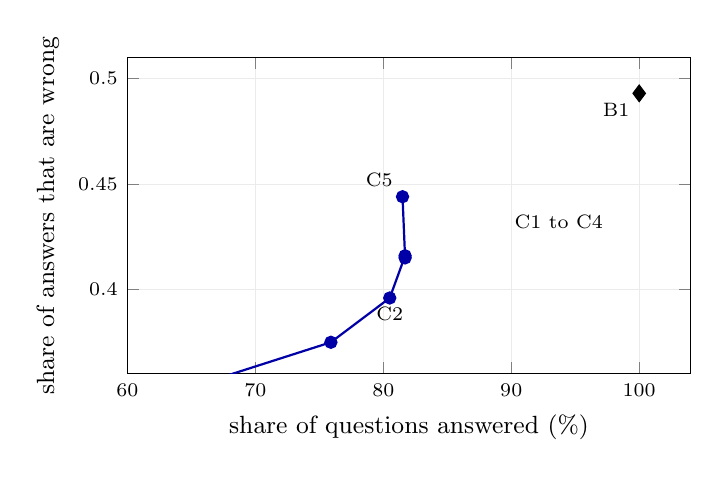
\begin{tikzpicture}
\begin{axis}[width=0.72\textwidth, height=5.6cm, xlabel={share of questions answered (\%)}, ylabel={share of answers that are wrong},
  xmin=60, xmax=104, ymin=0.36, ymax=0.51, font=\small, tick label style={font=\scriptsize}, grid=major, grid style={black!8}]
  \addplot[blue!65!black, mark=*, thick] coordinates {(34.2,0.294) (75.9,0.375) (80.5,0.396) (81.7,0.416) (81.7,0.415) (81.5,0.444)};
  \node[font=\scriptsize, anchor=south east] at (axis cs:34.2,0.294) {C0};
  \node[font=\scriptsize, anchor=north] at (axis cs:80.5,0.396) {C2};
  \node[font=\scriptsize, anchor=south east] at (axis cs:81.5,0.444) {C5};
  \node[font=\scriptsize, anchor=west] at (axis cs:89.5,0.432) {C1 to C4};
  \addplot[black, only marks, mark=diamond*, mark size=3pt] coordinates {(100,0.493)};
  \node[font=\scriptsize, anchor=north east] at (axis cs:100,0.493) {B1};
\end{axis}
\end{tikzpicture}
\caption[Answered share against error among answered.]{Selective-prediction view on the evaluation fold: share of questions answered and share of those answers that are wrong, for each cycle and for B1, which answers everything. CAEM stays below B1's error but answers more and errs more as the cycles go on.}
\label{fig:selective}
\end{figure}


\textbf{The status tag predicts correctness:} the user sees each answer with a status tag (\Cref{sec:setup-metrics}), and at every cycle verified answers are more often right than provisional ones, which in turn are more often right than conflicting or insufficient ones (\Cref{tab:status-tags}). Answers tagged verified are right $74.6$ percent of the time at C0, when a quarter of the questions receive that tag, and $65.5$ to $68.9$ percent at C1 to C5, when $42$ to $56$ percent do; provisional answers are right $40$ to $60$ percent of the time, and conflicting and insufficient ones $15$ to $48$ percent. B1 is right on $51.1$ percent of its answers and gives the user no signal of which ones. The tag is therefore the most direct user-facing benefit of the architecture: from C1 on, a user who acts only on verified answers meets about $30$ percent fewer wrong answers than one who trusts every answer of B1 (an error rate of $0.31$ to $0.35$ against $0.49$), at the cost of receiving a verified answer for only about half of the questions.

% Generated by scripts/build_final_tables.py from outputs/analysis/chm_judged.json (label em_final); do not edit.
\begin{table}[!htbp]
\centering\small
\setlength{\tabcolsep}{3.5pt}
\begin{tabular}{@{}lccccccccc@{}}
\toprule
 & \multicolumn{2}{c}{\textbf{Verified}} & \multicolumn{2}{c}{\textbf{Provisional}} & \multicolumn{2}{c}{\textbf{Conflicting}} & \multicolumn{2}{c}{\textbf{Insufficient}} & \\
\cmidrule(lr){2-3}\cmidrule(lr){4-5}\cmidrule(lr){6-7}\cmidrule(lr){8-9}
\textbf{Cycle} & \textbf{Share} & \textbf{EM} & \textbf{Share} & \textbf{EM} & \textbf{Share} & \textbf{EM} & \textbf{Share} & \textbf{EM} & \textbf{All} \\
\midrule
C0 & $24.9\%$ & $0.746$ & $9.3\%$ & $0.597$ & $31.9\%$ & $0.477$ & $33.9\%$ & $0.365$ & $0.517$ \\
C1 & $44.2\%$ & $0.689$ & $31.7\%$ & $0.535$ & $9.7\%$ & $0.219$ & $14.4\%$ & $0.264$ & $0.533$ \\
C2 & $46.8\%$ & $0.655$ & $33.6\%$ & $0.532$ & $7.3\%$ & $0.220$ & $12.3\%$ & $0.266$ & $0.535$ \\
C3 & $55.6\%$ & $0.668$ & $26.0\%$ & $0.403$ & $6.3\%$ & $0.326$ & $11.9\%$ & $0.151$ & $0.516$ \\
C4 & $55.3\%$ & $0.667$ & $26.3\%$ & $0.411$ & $6.6\%$ & $0.303$ & $11.7\%$ & $0.159$ & $0.517$ \\
C5 & $42.3\%$ & $0.667$ & $39.1\%$ & $0.433$ & $1.5\%$ & $0.217$ & $17.0\%$ & $0.306$ & $0.508$ \\
\bottomrule
\end{tabular}
\caption[Accuracy of the status tag shown to the user.]{Share of evaluation questions and EM for each status tag CAEM shows the user (verified: stored; provisional: deferred; conflicting: discarded, shown with a warning; insufficient: abstained, answer withheld), with EM over all questions for reference. B1, which shows no tag, has EM $0.511$.}
\label{tab:status-tags}
\end{table}


The retention ratios of every cycle are in \Cref{tab:sil-training-trajectory}: MMLU never comes near the floor (between $0.975$ and $1.041$); the TriviaQA test probe falls to $0.886$ at cycle four and triggers the only rollback. The composite evaluation score (\Cref{tab:ces-caem-trajectory} in \Cref{app:extra-tables}) rises from $0.585$ to $0.704$, mostly through its verifier-reliability axis, which grows with the calibration-fold separation $d$ (\Cref{tab:gate-quality}); its accuracy axis falls over the same cycles, so the rise in CES should not be read as a rise in accuracy.

\subsubsection{Per-benchmark trajectory}
\label{sec:headline-per-bench}

\Cref{tab:per-bench-trajectory} and \Cref{tab:halluc-subtypes} break the pooled numbers down. On the training panel, FEVER and TriviaQA peak at C1 or C2 (FEVER $0.533$ against B1's $0.507$; TriviaQA $0.493$ against $0.430$) and fall back afterwards, FEVER to $0.477$, below B1, and TriviaQA to $0.453$, still above it. CommonsenseQA is highest at C0 ($0.757$ against $0.727$) and ends at $0.717$. TriviaQA is the benchmark where the architecture helps most and where the verifier separates correct from incorrect answers best (\Cref{sec:disc-verifier-scope}); even there, the C2 gain over B1 is not significant at $300$ questions. On the transfer panel, TruthfulQA stays between $0.230$ and $0.277$ at every cycle against B1's $0.250$, and StrategyQA between $0.610$ and $0.653$ against $0.643$. Across subtypes, factual and logical fabrication fall gently after C0; defensive evasion and over-long output are near zero. Template leakage is zero for every cycle and every baseline, and this is a real zero: the answer prompt shows the reasoning line as a bracketed placeholder, and no system ever copied a placeholder into its output.

% Table sizing standardised 2026-10-17 (final drafting pass): \small, no \resizebox.
% Caption shortened by hand in the final drafting pass (2026-10); detail moved to chapter 5 text.
% Auto-generated by scripts/aggregate_section_5_2.py
% Per-cycle, per-benchmark EM (top sub-row) and CHM (bottom sub-row),
% with training-panel pooled rows merged in (previously tab:train-vs-transfer),
% the no-CAEM reference floor (B1 zero-shot) on the left, and absolute +
% relative deltas against the best CAEM cycle (C2) and the trajectory final
% cycle (C5) on the right.
% Transfer panel intentionally has no pooled row: TruthfulQA and StrategyQA
% move in opposite directions and any pooled average is dishonest reporting.
\begin{table}[!htbp]
\centering\small
\setlength{\tabcolsep}{3pt}
\begin{tabular}{@{}lccccccccc@{}}
\toprule
\textbf{Benchmark} & \textbf{B1} & \textbf{C0} & \textbf{C1} & \textbf{C2} & \textbf{C3} & \textbf{C4} & \textbf{C5} & \twoline{Change\\to C2} & \twoline{Change\\to C5} \\
\midrule
\multicolumn{10}{@{}l}{\textit{Training panel}} \\
FEVER (EM) & 0.453 & 0.487 & 0.533 & 0.533 & 0.503 & 0.507 & 0.477 & $+0.080$ & $+0.024$ \\
FEVER (CHM) & 0.159 & 0.139 & 0.113 & 0.102 & 0.120 & 0.119 & 0.126 & $-0.057$ & $-0.033$ \\
TriviaQA (EM) & 0.293 & 0.463 & 0.480 & 0.493 & 0.463 & 0.463 & 0.453 & $+0.200$ & $+0.160$ \\
TriviaQA (CHM) & 0.175 & 0.156 & 0.113 & 0.109 & 0.121 & 0.120 & 0.125 & $-0.066$ & $-0.050$ \\
CSQA (EM) & 0.703 & 0.763 & 0.740 & 0.717 & 0.743 & 0.743 & 0.717 & $+0.014$ & $+0.014$ \\
CSQA (CHM) & 0.096 & 0.077 & 0.086 & 0.093 & 0.086 & 0.085 & 0.091 & $-0.003$ & $-0.005$ \\
\rowcolor{gray!18}
\textbf{Pooled (EM)} & $\mathbf{0.483}$ & $0.571$ & $0.584$ & $\mathbf{0.581}$ & $0.570$ & $0.571$ & $0.549$ & $\mathbf{+0.098}$ & $\mathbf{+0.066}$ \\
\rowcolor{gray!18}
\textbf{Pooled (CHM)} & $\mathbf{0.143}$ & $0.124$ & $0.104$ & $\mathbf{0.101}$ & $0.109$ & $0.108$ & $0.114$ & $\mathbf{-0.042}$ & $\mathbf{-0.029}$ \\
\midrule
\multicolumn{10}{@{}l}{\textit{Transfer panel}} \\
TruthfulQA (EM) & 0.433 & 0.380 & 0.317 & 0.323 & 0.310 & 0.307 & 0.300 & $-0.110$ & $-0.133$ \\
TruthfulQA (CHM) & 0.051 & 0.150 & 0.133 & 0.116 & 0.119 & 0.122 & 0.104 & $+0.065$ & $+0.053$ \\
StrategyQA (EM) & 0.650 & 0.610 & 0.647 & 0.653 & 0.640 & 0.640 & 0.640 & $+0.003$ & $-0.010$ \\
StrategyQA (CHM) & 0.120 & 0.154 & 0.113 & 0.115 & 0.128 & 0.127 & 0.099 & $-0.005$ & $-0.021$ \\
\bottomrule
\end{tabular}
\caption[EM and CHM by benchmark and cycle.]{EM (upper row) and CHM (lower row) by benchmark and cycle on the evaluation fold, with B1 and the change from B1 to C2 and C5. Shaded rows pool the training panel; the transfer panel is not pooled because its two benchmarks move in opposite directions.}
\label{tab:per-bench-trajectory}
\end{table}


% CHM cells re-scored (Haiku-judged TruthfulQA; mean of the seven active types) by scripts/patch_chm_judged_tables.py (2026-10-17).
% CHM cells re-scored with the Haiku-judged TruthfulQA label by scripts/patch_chm_judged_tables.py (2026-10-17).
% Table sizing standardised 2026-10-17 (final drafting pass): \small, no \resizebox.
% Caption shortened by hand in the final drafting pass (2026-10); detail moved to chapter 5 text.
% Auto-generated by scripts/aggregate_section_5_2.py
% Per-cycle pooled per-subtype CHM rates with B1 reference column.
% Pool = all 1500 samples (5 benches x 300) per cycle.
% B1 column from outputs/baselines_phase1e/chm_comparison.json (zero_shot).
\begin{table}[!htbp]
\centering\small
\setlength{\tabcolsep}{5pt}
\begin{tabular}{lccccccc}
\toprule
\textbf{Subtype} & \textbf{B1 ref} & \textbf{C0} & \textbf{C1} & \textbf{C2} & \textbf{C3} & \textbf{C4} & \textbf{C5} \\
\midrule
Conf.\ confab. & 0.327 & 0.088 & 0.238 & 0.259 & 0.291 & 0.289 & 0.307 \\
Fact.\ fabric. & 0.381 & 0.361 & 0.327 & 0.314 & 0.319 & 0.319 & 0.316 \\
Logic.\ fabric. & 0.307 & 0.281 & 0.265 & 0.245 & 0.278 & 0.275 & 0.238 \\
Def.\ evasion & 0.019 & 0.044 & 0.009 & 0.006 & 0.002 & 0.002 & 0.003 \\
Templ.\ leak & 0.000 & 0.000 & 0.000 & 0.000 & 0.000 & 0.000 & 0.000 \\
False refusal & 0.055 & 0.298 & 0.069 & 0.057 & 0.054 & 0.053 & 0.065 \\
Over-long & 0.005 & 0.000 & 0.001 & 0.003 & 0.005 & 0.005 & 0.004 \\
\midrule
\textbf{CHM (mean of 7)} & \textbf{0.156} & 0.153 & 0.130 & 0.126 & 0.135 & 0.135 & 0.133 \\
\bottomrule
\end{tabular}
\caption[The seven hallucination subtypes by cycle.]{The seven subtypes of the composite hallucination metric (\Cref{sec:setup-metrics}) by cycle, pooled over the evaluation fold ($1{,}500$ questions), with B1 for reference.}
\label{tab:halluc-subtypes}
\end{table}


\FloatBarrier

\subsubsection{Training versus transfer contrast}
\label{sec:headline-id-vs-transfer}

On the training panel, whose benchmarks feed the calibration fold and the training pool, CAEM gains a little and then loses it: EM $0.554$ (B1) against $0.581$ at C2 and $0.549$ at C5, and CHM $0.126$ against $0.116$ and $0.130$. The transfer panel, which the system never trains on, shows no gain at any cycle: TruthfulQA EM is $0.253$ at C5 against $0.250$ for B1, with a higher CHM ($0.168$ against $0.147$), and StrategyQA EM $0.640$ against $0.643$, with a lower CHM ($0.113$ against $0.137$). Self-improvement therefore did not damage the transfer benchmarks, but it did not carry over to them either.

\subsection{Four-outcome decision distribution}
\label{sec:decision-distribution}

The three readings in this subsection use three different folds, named in each paragraph; the second and third tables are in \Cref{app:extra-tables}.

\textbf{On the calibration fold} (\Cref{tab:decision-distribution}), the share stored rises from $42$ percent at C1 to $59$ percent at C5, deferral from $12$ to $29$ percent, while discard falls from $25$ to $3$ percent and abstention from $21$ to $10$ percent. The outcomes are ordered by correctness at every cycle: stored answers are right $73$ to $75$ percent of the time, deferred ones less, discarded ones less again, and abstentions least ($0.38$ at C1, $0.17$ at C5). The gap between stored and the next outcome widens from $14$ points at C1 to between $24$ and $30$ points afterwards.

% Table sizing standardised 2026-10-17 (final drafting pass): \small, no \resizebox.
% Caption shortened by hand in the final drafting pass (2026-10); detail moved to chapter 5 text.
% Auto-generated by scripts/aggregate_section_5_3.py
% Hand-corrected 2026-10-15 (see ref_check/fixes_applied.md)
% Panel (b) source: outputs/full_run/cycle_3/calibration/{fever,triviaqa,commonsense_qa}_cycle3.json,
% same computation as panel (a) (samples without a gate decision excluded: 6/1/4).
% Per-cycle four-outcome decision distribution on the training-panel calibration fold.
% Cycles 1,2,3,5 only (C0 is cold-start before first calibration; C4 was aborted under retention guard).
% Per-benchmark snapshot reported at the cycle-three anchor.
\begin{table}[!htbp]
\centering\small
\setlength{\tabcolsep}{3pt}
\begin{tabular}{lcccccccc}
\toprule
 & \multicolumn{2}{c}{\textbf{Store}} & \multicolumn{2}{c}{\textbf{Defer}} & \multicolumn{2}{c}{\textbf{Discard}} & \multicolumn{2}{c}{\textbf{Abstain}} \\
\cmidrule(lr){2-3}\cmidrule(lr){4-5}\cmidrule(lr){6-7}\cmidrule(lr){8-9}
 & share & EM & share & EM & share & EM & share & EM \\
\midrule
\multicolumn{9}{@{}l}{\textit{(a) Pooled training panel}} \\
C1 & 42.1\% & 0.74 & 12.0\% & 0.60 & 25.0\% & 0.58 & 20.9\% & 0.38 \\
C2 & 67.2\% & 0.74 & 18.7\% & 0.44 & 5.4\% & 0.38 & 8.7\% & 0.25 \\
C3 & 60.4\% & 0.75 & 26.0\% & 0.47 & 5.5\% & 0.41 & 8.1\% & 0.22 \\
C5 & 58.6\% & 0.73 & 28.5\% & 0.49 & 3.4\% & 0.46 & 9.5\% & 0.17 \\
\midrule
\multicolumn{9}{@{}l}{\textit{(b) By benchmark at C3 ($500$ each)}} \\
FEVER & 55.1\% & 0.76 & 38.1\% & 0.47 & 4.3\% & 0.52 & 2.6\% & 0.38 \\
TriviaQA & 40.5\% & 0.79 & 28.9\% & 0.45 & 10.6\% & 0.30 & 20.0\% & 0.17 \\
CommonsenseQA & 85.7\% & 0.72 & 11.1\% & 0.55 & 1.6\% & 0.88 & 1.6\% & 0.62 \\
\bottomrule
\end{tabular}
\caption[Decision shares on the calibration fold.]{Share of each decision and the EM within it on the training-panel calibration fold: (a) pooled by cycle; (b) per benchmark at cycle three. C0 and the rolled-back C4 have no reading.}
\label{tab:decision-distribution}
\end{table}


\textbf{On the stream chunks and the transfer evaluation folds} (\Cref{tab:decision-matrix-trajectory}), stored answers are more often correct than deferred ones in every row. The full ordering stored, deferred, discarded holds in half the rows; where it fails, the discard class is small. On TruthfulQA, stored answers are right only $31$ to $38$ percent of the time at C1 to C5, far below the training panel.

\textbf{On the evaluation fold} (\Cref{tab:abstention-per-bench}), FEVER abstention falls from $64.3$ percent at C0 to $5.3$ percent at C5; CommonsenseQA almost never abstains, because a multiple-choice prompt forces an answer; TruthfulQA abstains on $23$ to $33$ percent of questions, a rate that falls slightly over the cycles while its EM stays flat; StrategyQA swings between $2$ and $43$ percent.

\FloatBarrier

\subsection{Three-tier router efficiency}
\label{sec:tier-efficiency}

\subsubsection{Per-tier hit rate trajectory and per-tier exact match}
\label{sec:tier-hit}

The design expects the memory-direct share to grow as the memory fills and the zero-shot share to grow as fine-tuning folds retrieved knowledge into the generator. Neither happened on the evaluation fold (\Cref{tab:tier-trajectory}). Tier 1 answered $7$ of the $9{,}000$ evaluation queries over six cycles, because every stream chunk and the evaluation fold share no question with the stored episodes; all seven answers were correct, and a direct probe of the router answered $42$ of $50$ exact repeats and $19$ of $50$ paraphrases of stored questions, $41$ and $19$ of them correctly (\Cref{tab:tier1-probe}). Tier 1 is built for deployment, where users repeat questions; this study used fresh questions to measure learning, so the probe is the test of this tier. Because a repeated question receives an answer that has already passed the storage gate, both exact match and the composite hallucination metric are expected to improve in deployment as the share of repeated questions grows. The zero-shot share moved from $48.7$ percent at C0 to $50.2$ percent at C5, peaking at $55.2$ percent at C2.

Within tiers, zero-shot answers are more accurate than retrieval-augmented ones at every cycle ($0.565$ against $0.472$ at C0, $0.519$ against $0.495$ at C5; \Cref{tab:tier-chm-trajectory} in \Cref{app:extra-tables}). At C0 this holds on four of five benchmarks, with TriviaQA the exception (\Cref{tab:per-tier-em}). Part of the difference is selection: the router and the classifier send to Tier 2 the questions they judge the generator can already answer. The zero-shot tier's accuracy also falls over the cycles, which is where the self-improvement loop acts.

% Auto-generated by scripts/build_ch5_evidence_tables.py from outputs/tier1_routing_probe/
% (results_cycle5.json, em_analysis.json). The probe's top1_is_source_rate field is not used:
% it compares two different id spaces (see ref_check/REPO_CLEANUP_TRACKER.md, C2).
\begin{table}[!htbp]
\centering\small
\begin{tabular}{@{}lrrrrrr@{}}
\toprule
 & \multicolumn{3}{c}{\textbf{Exact repeats}} & \multicolumn{3}{c}{\textbf{Paraphrases}} \\
\cmidrule(lr){2-4}\cmidrule(l){5-7}
\textbf{Source benchmark} & Asked & Tier 1 & Correct & Asked & Tier 1 & Correct \\
\midrule
FEVER & $17$ & $13$ & $13$ & $17$ & $7$ & $7$ \\
TriviaQA & $23$ & $22$ & $22$ & $23$ & $12$ & $12$ \\
CommonsenseQA & $10$ & $7$ & $6$ & $10$ & $0$ & $0$ \\
\midrule
\textbf{Total} & $50$ & $42$ & $41$ & $50$ & $19$ & $19$ \\
\bottomrule
\end{tabular}
\caption[Router probe of the memory-direct tier.]{Router probe of the memory-direct tier at cycle five: $50$ stored questions asked again word for word and $50$ asked as paraphrases. Tier 1 counts the questions answered from memory; Correct counts those answers that match the gold answer.}
\label{tab:tier1-probe}
\end{table}


% Generated by scripts/build_final_tables.py from outputs/analysis/chm_judged.json (label em_final); do not edit.
\begin{table}[!htbp]
\centering\small
\setlength{\tabcolsep}{4pt}
\begin{tabular}{@{}lccccccc@{}}
\toprule
  & \multicolumn{2}{c}{\twoline{Tier 1\\(memory)}} & \multicolumn{2}{c}{\twoline{Tier 2\\(zero-shot)}} & \multicolumn{2}{c}{\twoline{Tier 3\\(RAG)}} & \\
 & share & EM & share & EM & share & EM & \twoline{Pooled\\EM} \\
\midrule
\multicolumn{8}{@{}l}{\textit{(a) Pooled over the five benchmarks}} \\
C0 & 0.0\% & -- & 48.7\% & 0.565 & 51.3\% & 0.472 & 0.517 \\
C1 & 0.0\% & -- & 49.8\% & 0.566 & 50.2\% & 0.501 & 0.533 \\
C2 & 0.1\% & 1.000 & 55.2\% & 0.548 & 44.7\% & 0.517 & 0.535 \\
C3 & 0.1\% & 1.000 & 44.7\% & 0.532 & 55.1\% & 0.502 & 0.516 \\
C4 & 0.1\% & 1.000 & 45.6\% & 0.532 & 54.3\% & 0.502 & 0.517 \\
C5 & 0.1\% & 1.000 & 50.2\% & 0.519 & 49.7\% & 0.495 & 0.508 \\
\midrule
\multicolumn{8}{@{}l}{\textit{(b) By benchmark at C5 ($300$ each)}} \\
FEVER & 0.0\% & -- & 43.3\% & 0.500 & 56.7\% & 0.459 & 0.477 \\
TriviaQA & 0.3\% & 1.000 & 37.0\% & 0.423 & 62.7\% & 0.468 & 0.453 \\
CommonsenseQA & 0.0\% & -- & 82.3\% & 0.745 & 17.7\% & 0.585 & 0.717 \\
TruthfulQA & 0.3\% & 1.000 & 64.3\% & 0.254 & 35.3\% & 0.245 & 0.253 \\
StrategyQA & 0.0\% & -- & 24.0\% & 0.639 & 76.0\% & 0.640 & 0.640 \\
\bottomrule
\end{tabular}
\caption[Tier shares and per-tier EM by cycle.]{Share of evaluation queries sent to each tier and the EM within it: (a) pooled by cycle; (b) per benchmark at C5.}
\label{tab:tier-trajectory}
\end{table}


\subsubsection{Per-tier latency and cost}
\label{sec:tier-cost}

The mean time per evaluation query, from the batched evaluation log, stays between $13.6$ and $14.7$ seconds per query (about six hours per cycle for the $1{,}500$ evaluation questions), as expected when the tier shares hardly move. This is about a hundred times slower than B1 ($142$ milliseconds), because every generated answer passes through the verifier's resampling, retrieval and entailment steps. Per benchmark at C5, CommonsenseQA is fastest ($8.6$ seconds) and TruthfulQA slowest ($17.8$ seconds). The time per tier could not be separated from the batched log, so the deployment-cost model of \Cref{eq:deployment-cost} cannot be filled in tier by tier; given the flat tier shares, it would predict a flat cost in any case.

\subsubsection{Why the safety override fires}
\label{sec:tier-safety}

The safety override fired on $63$ of the $9{,}000$ evaluation queries ($0.7$ percent) and on $3$ of the $23{,}500$ stream-chunk queries. Of the evaluation firings, $62$ were CommonsenseQA questions after that benchmark's floor was refitted from $0.38$ to $0.491$ at cycle three and $0.569$ at cycle five; the other was one StrategyQA question at cycle five. On FEVER and TriviaQA the override never fired, because their pre-routing temperature reached its upper bound and pulled $\upre$ toward $0.5$ (\Cref{sec:pre-routing}). The override therefore acted as a rarely used safeguard in this run, not as an active part of routing.

\FloatBarrier

\subsection{Retention and continual learning}
\label{sec:retention}

The retention guard reads three probes after every fine-tune (\Cref{tab:sil-training-trajectory}). It kept cycles one, two, three and five, and rolled back cycle four, when the TriviaQA test ratio fell to $0.886$; the memory was kept and grew across the rollback. On the benchmarks themselves, CommonsenseQA lost $4.0$ points and FEVER $1.0$ point from C0 to C5, and both fell further from their peaks (\Cref{tab:per-bench-trajectory}); the probe panel did not catch these losses because the CommonsenseQA probe stayed above its floor and FEVER is not probed. The training set grew from $107$ episodes at the first fine-tune to $5{,}006$ at the last, and the final training loss fell from $0.258$ to $0.070$ over cycles one to four, then rose to $0.091$ at cycle five after training restarted from the cycle-three adapter (\Cref{tab:sil-training-trajectory}).

% Caption shortened by hand in the final drafting pass (2026-10); detail moved to chapter 5 text.
% Auto-generated from outputs/full_run/retroverify_cycle*.json::fine_tune
% + outputs/full_run/all_cycle_results.json (multi-modal retention probes).
% Per-cycle SIL training trajectory: episode count, final training loss,
% three-probe retention panel (MMLU + TQA-test + CSQA-test), rollback status.
\begin{table}[H]
\centering\footnotesize
\setlength{\tabcolsep}{6pt}
\resizebox{\textwidth}{!}{%
\begin{tabular}{@{}lrrrrrl@{}}
\toprule
 & & & \multicolumn{3}{c}{\textbf{Retention probe ratio}} & \\
\cmidrule(lr){4-6}
\textbf{Cycle} & $\boldsymbol{n_{\text{episodes used}}}$ & \textbf{Final loss} & \textbf{MMLU} & \textbf{TQA-test} & \textbf{CSQA-test} & \textbf{Outcome} \\
\midrule
C1 & $107$ & $0.258$ & $1.041$ & $1.013$ & $1.006$ & commit \\
C2 & $1\,474$ & $0.171$ & $0.975$ & $0.949$ & $0.982$ & commit \\
C3 & $2\,966$ & $0.109$ & $0.992$ & $0.987$ & $0.976$ & commit \\
C4 & $3\,624$ & $0.070$ & $1.018$ & $\mathbf{0.886}^{\dagger}$ & $0.982$ & abort (retention rollback) \\
C5 & $5\,006$ & $0.091$ & $0.999$ & $1.013$ & $0.958$ & commit (post-rollback recovery) \\
\bottomrule
\multicolumn{7}{@{}l}{\footnotesize $^{\dagger}$ Cycle-four TriviaQA-test ratio of $0.886$ crossed below the registered floor of $\rho_{\min} = 0.93$, triggering the asymmetric rollback.} \\
\end{tabular}%
}
\caption[Self-improvement training by cycle.]{Episodes used for fine-tuning, final training loss and retention ratios by cycle.}
\label{tab:sil-training-trajectory}
\end{table}


\FloatBarrier

\subsection{Memory and training-pool dynamics}
\label{sec:pool-dynamics}

\textbf{Memory growth:} the memory grew from the $431$ gold-filtered cold-start entries to $12{,}175$ at C5, adding between $2{,}214$ and $2{,}484$ entries per cycle, including the rolled-back cycle four; the deferred buffer grew to $4{,}284$ entries (\Cref{tab:memory-store-trajectory}).

% Hand-merged 2026-10-17 (final drafting pass, ch5 table reduction) from three committed tables:
% tab_memory_store_trajectory.tex (memory, deferred buffer, change), tab_survival_distribution.tex
% (promoted, TTL-dropped) and tab_consolidation_trajectory.tex (groups merged, entries removed).
% Values copied unchanged; logged in ref_check/fixes_applied.md and REPO_CLEANUP_TRACKER.md (T10).
\begin{table}[!htbp]
\centering\small
\setlength{\tabcolsep}{4pt}
\begin{tabular}{@{}lrrrrrrr@{}}
\toprule
 & \multicolumn{2}{c}{\textbf{Memory}} & \multicolumn{3}{c}{\textbf{Deferred buffer}} & \multicolumn{2}{c}{\textbf{Consolidation}} \\
\cmidrule(lr){2-3}\cmidrule(lr){4-6}\cmidrule(lr){7-8}
\textbf{Cycle} & \textbf{Entries} & \textbf{Change} & \textbf{Entries} & \textbf{Promoted} & \textbf{Dropped} & \textbf{Merged} & \textbf{Removed} \\
\midrule
C0 & $431$ & --- & $0$ & --- & --- & --- & --- \\
C1 & $2\,818$ & $+2\,387$ & $1\,123$ & $0$ & $0$ & $0$ & $0$ \\
C2 & $5\,151$ & $+2\,333$ & $2\,399$ & $131$ & $0$ & $3$ & $3$ \\
C3 & $7\,477$ & $+2\,326$ & $2\,692$ & $220$ & $924$ & $11$ & $11$ \\
C4$^{\ast}$ & $9\,961$ & $+2\,484$ & $4\,068$ & --- & --- & --- & --- \\
C5 & $12\,175$ & $+2\,214$ & $4\,284$ & $299$ & $1\,169$ & $43$ & $44$ \\
\midrule
Total & & & & $650$ & $2\,093$ & $57$ & $58$ \\
\bottomrule
\end{tabular}
\caption[Memory, deferred buffer and consolidation by cycle.]{Memory and deferred-buffer size at the close of each cycle, answers promoted from or dropped by the buffer, and near-duplicate groups merged. $^{\ast}$Cycle four was rolled back, so its reconsideration and consolidation passes were skipped.}
\label{tab:memory-store-trajectory}
\end{table}


\textbf{Training pool:} the training threshold ($\ustored \ge 0.70$) keeps a purer subset of the stored answers (\Cref{tab:storage-pool-quality}). On the stream chunks, the training pool is $79.8$ to $81.8$ percent correct, against $72.4$ to $75.3$ percent for everything stored, so the stricter threshold removes between $56$ and $73$ percent of the wrong stored answers before training. About a fifth of the training pool is still wrong. Stored scores are well ordered against correctness on the stream chunks at every cycle, but on the evaluation fold only at cycles one and four (\Cref{tab:u-stored-distribution} in \Cref{app:extra-tables}).

% Table sizing standardised 2026-10-17 (final drafting pass): \small, no \resizebox.
% Caption shortened by hand in the final drafting pass (2026-10); detail moved to chapter 5 text.
% Auto-generated from outputs/full_run/eval/{bench}_cycle{c}.json,
% outputs/full_run/eval/{bench}_cycle{c}_streamchunk.json, retroverify_cycle*.json
% Stored-episode em-correctness, training-threshold filter, SIL pool purity, and
% SIL training-batch size per cycle, reported on both the held-out evaluation fold
% (panel a) and the SIL stream chunks (panel b, the production candidate pool).
% Hand-corrected 2026-10-15 (see ref_check/fixes_applied.md)
\begin{table}[!htbp]
\centering\small
\setlength{\tabcolsep}{4pt}
\begin{tabular}{@{}lrrrrrrrr@{}}
\toprule
\textbf{Cycle} & $\boldsymbol{n_{\text{stored}}}$ & \textbf{Correct} & \textbf{Wrong} & $\boldsymbol{\pi_{\text{store}}}$ & \twoline{Above\\$\boldsymbol{\tau_{\text{train}}}$} & \twoline{Share\\above} & $\boldsymbol{\pi_{\text{SIL}}}$ & \twoline{Used in\\training} \\
\midrule
\multicolumn{9}{@{}l}{\textit{(a) Evaluation fold}} \\
C0 & $336$ & $255$ & $81$  & $0.759$ & $58$  & $17.3\%$ & $0.793$ & --- \\
C1 & $515$ & $374$ & $141$ & $0.726$ & $231$ & $44.9\%$ & $0.788$ & --- \\
C2 & $534$ & $370$ & $164$ & $0.693$ & $266$ & $49.8\%$ & $0.726$ & --- \\
C3 & $565$ & $402$ & $163$ & $0.712$ & $279$ & $49.4\%$ & $0.735$ & --- \\
C4$^{\ast}$ & $566$ & $402$ & $164$ & $0.710$ & $272$ & $48.1\%$ & $0.735$ & --- \\
C5 & $504$ & $353$ & $151$ & $0.700$ & $181$ & $35.9\%$ & $0.735$ & --- \\
\midrule
\multicolumn{9}{@{}l}{\textit{(b) Stream chunks}} \\
C1 & $2\,456$ & $1\,850$ & $606$ & $0.753$ & $1\,309$ & $53.3\%$ & $0.818$ & $107$ \\
C2 & $2\,494$ & $1\,873$ & $621$ & $0.751$ & $1\,448$ & $58.1\%$ & $0.810$ & $1\,474$ \\
C3 & $2\,490$ & $1\,802$ & $688$ & $0.724$ & $1\,337$ & $53.7\%$ & $0.798$ & $2\,966$ \\
C4$^{\ast}$ & $2\,522$ & $1\,862$ & $660$ & $0.738$ & $1\,413$ & $56.0\%$ & $0.803$ & --- \\
C5 & $2\,380$ & $1\,724$ & $656$ & $0.724$ & $895$ & $37.6\%$ & $0.803$ & $5\,006$ \\
\bottomrule
\end{tabular}
\par\vspace{2pt}{\footnotesize\parbox{\linewidth}{$^{\ast}$Cycle four was rolled back, so its training pool is not reported.}\par}
\caption[Stored answers and the training pool by cycle.]{Stored answers, their precision, the share passing the training threshold ($\ustored \ge 0.70$) and the precision of that training pool, on (a) the evaluation fold and (b) the stream chunks.}
\label{tab:storage-pool-quality}
\end{table}


\textbf{Re-verification and deferral:} reconstructing the memory snapshots identifies $1{,}094$ entries removed by the retroactive pass (the run log counts $1{,}061$); $38.4$ percent of them were wrong, against about $22$ percent in the pool, so the pass removes wrong entries at about $1.75$ times their base rate (\Cref{tab:em-conditional-breakdown} in \Cref{app:extra-tables}). The deferred buffer promoted $650$ answers ($131$, $220$ and $299$ at cycles two, three and five, \Cref{tab:memory-store-trajectory}); of the $620$ promotions recovered from the snapshots, $55.6$ percent were correct, which is below the stored pool but means about $345$ correct answers rescued from the deferral band. Consolidation merged $57$ groups and removed $58$ entries (\Cref{tab:memory-store-trajectory}); its same-answer guard blocked several merges of near-identical questions with different answers.

\FloatBarrier

\subsection{Theoretical predictions checked against the trajectory}
\label{sec:theory-checks}

This subsection reads the statements of \Cref{sec:theory} against the run. The two proven results are checked against their assumptions; the heuristics and remarks are read as consistency checks. \Cref{tab:theorem-receipts-summary} summarises the readings.

% Auto-generated by scripts/build_ch5_evidence_tables.py (final drafting pass, 2026-10).
\begin{table}[!htbp]
\centering\small
\setlength{\tabcolsep}{4pt}
\begin{tabular}{@{}lrrrrrrrrr@{}}
\toprule
 & \multicolumn{6}{c}{\textbf{Pooled training panel}} & \multicolumn{3}{c}{\textbf{Balanced accuracy}} \\
\cmidrule(lr){2-7}\cmidrule(l){8-10}
\textbf{Cycle} & \textbf{Stored} & \textbf{Precision} & \textbf{TPR} & \textbf{FPR} & \textbf{Bal.\ acc.} & \textbf{Cohen's $d$} & \textbf{FEVER} & \textbf{TriviaQA} & \textbf{CSQA} \\
\midrule
C0$^{\ast}$ & $560$ (37.3\%) & $0.780$ & $0.653$ & $0.148$ & $0.753$ & $1.468$ & -- & -- & -- \\
C1 & $630$ (42.0\%) & $0.740$ & $0.510$ & $0.280$ & $0.615$ & $0.593$ & $0.665$ & $0.500$ & $0.522$ \\
C2 & $1001$ (66.7\%) & $0.736$ & $0.791$ & $0.465$ & $0.663$ & $0.773$ & $0.672$ & $0.689$ & $0.554$ \\
C3 & $899$ (59.9\%) & $0.746$ & $0.725$ & $0.397$ & $0.664$ & $0.756$ & $0.653$ & $0.719$ & $0.531$ \\
C5 & $868$ (57.9\%) & $0.732$ & $0.705$ & $0.389$ & $0.658$ & $0.842$ & $0.633$ & $0.687$ & $0.550$ \\
\bottomrule
\end{tabular}
\caption[Storage gate quality on the calibration fold by cycle.]{Storage gate quality on the training-panel calibration fold ($1{,}500$ questions) by cycle. $^{\ast}$C0 is in-sample (the composite was fitted on this fold); C1 to C5 score the fold with the new adapter before the composite is refitted. C4 was rolled back and has no reading.}
\label{tab:gate-quality}
\end{table}


\subsubsection{Pool purity}
\label{sec:check-purity}

\textbf{Pool purity floor:} the floor of \Cref{thm:purity} depends on new entries being as often correct as the calibration fold at the same cut-point (assumption (ii)). On the training panel this approximately held: the calibration-fold precision at $\tau_{\text{store}} = 0.60$ was between $0.732$ and $0.746$ at C1 to C5 (\Cref{tab:pi-store-trajectory}), and the answers actually stored from each stream chunk were $0.753$, $0.751$, $0.724$, $0.738$ and $0.724$ correct. On the evaluation fold the pooled storage precision was between $0.693$ and $0.756$; FEVER's own evaluation-fold precision was lower, between $0.614$ and $0.634$ at C1 to C4 and $0.649$ at C5, which shows that the pooled statement does not carry over to every benchmark. On TruthfulQA, where the questions are unlike the calibration fold, the assumption failed: stored answers were right only $31$ to $38$ percent of the time.

% C0 cal-fold cell and caption hand-corrected in the final drafting pass (2026-10).
% Auto-generated by scripts/aggregate_pi_store_trajectory.py
% Per-cycle empirical storage precision π_store at τ_store = 0.60
% Reports both calibration-fold (theorem-anchored) and evaluation-fold
% (deployment-realised) readings; cycle four has no cal-fold refit but the
% eval-fold reading is computed against the rolled-back C3 composite.
\begin{table}[H]
\centering\footnotesize
\setlength{\tabcolsep}{4pt}
\resizebox{\textwidth}{!}{%
\begin{tabular}{@{}l|cc|cc|ccc@{}}
\toprule
 & \multicolumn{2}{c|}{\textbf{Cal-fold pooled}} & \multicolumn{2}{c|}{\textbf{Eval-fold pooled}} & \multicolumn{3}{c}{\textbf{Eval-fold per-bench $\pi_{\text{store}}$}} \\
\textbf{Cycle} & $n$ & $\pi_{\text{store}}$ & $n$ & $\pi_{\text{store}}$ & FEVER & TriviaQA & CSQA \\
\midrule
C0 & $560$ & $0.780^{\dagger}$ & $336$ & $0.759$ & $0.661$ & --- & $0.779$ \\
C1 & $631$ & $0.740$ & $515$ & $0.726$ & $0.634$ & $0.797$ & $0.736$ \\
C2 & $1\,001$ & $0.736$ & $534$ & $0.693$ & $0.630$ & $0.733$ & $0.705$ \\
C3 & $899$ & $0.746$ & $565$ & $0.712$ & $0.617$ & $0.741$ & $0.750$ \\
C4$^{\ast}$ & --- & --- & $566$ & $0.710$ & $0.614$ & $0.733$ & $0.754$ \\
C5 & $868$ & $0.732$ & $504$ & $0.700$ & $0.649$ & $0.704$ & $0.725$ \\
\bottomrule
\multicolumn{8}{@{}l}{\footnotesize $^{\dagger}$ In-sample: the cycle-zero composite was fitted on this fold (re-run sweep, locked configuration).} \\
\multicolumn{8}{@{}l}{\footnotesize $^{\ast}$ Cycle four was aborted under the retention guard; the cal-fold refit was skipped, but the eval-fold reading is computed against the rolled-back C3 composite.} \\
\end{tabular}%
}
\caption[Storage precision by cycle on the calibration and evaluation folds.]{Storage precision $\pi_{\text{store}}$ at $\tau_{\text{store}} = 0.60$ by cycle: share of stored answers that are correct, on the training-panel calibration fold and on the evaluation fold.}
\label{tab:pi-store-trajectory}
\end{table}


\textbf{Purification condition (H1):} the gate purifies only if its balanced accuracy exceeds one half (\Cref{thm:bayes-purity}). Pooled over the training panel it was $0.615$, $0.663$, $0.664$ and $0.658$ at C1, C2, C3 and C5 (\Cref{tab:gate-quality}), measured with the new adapter before each refit; the C0 value of $0.753$ is in-sample. The weakest benchmarks were CommonsenseQA ($0.52$ to $0.55$) and TriviaQA at C1, where the gate stored no TriviaQA answer and the balanced accuracy is exactly $0.500$.

\subsubsection{Monotonicity}
\label{sec:check-monotonicity}

\Cref{thm:monotone} predicts that better separation stores more answers when the correct class is denser at the cut-point. The separation $d$ rose from $0.593$ at C1 to $0.773$ at C2 while the share stored rose from $0.420$ to $0.667$, as predicted; from C2 to C3, $d$ was flat ($0.756$) and the share fell to $0.599$; from C3 to C5, $d$ rose to $0.842$ while the share fell to $0.579$ (\Cref{tab:gate-quality}). Only the first step agrees. The refit of the composite at every cycle, which the heuristic does not model, is the most likely reason; separating the two would need a cycle with the composite frozen (\Cref{ch:conclusion}).

\subsubsection{Convergence}
\label{sec:check-convergence}

\textbf{Convergence envelope (H3):} the calibration-fold precision stayed between $0.732$ and $0.746$ at C1 to C5, a band of width $0.014$ (\Cref{tab:pi-store-trajectory}). For about $900$ stored answers per cycle, the standard error of one reading is about $0.015$, so the band is as narrow as sampling noise allows; six cycles cannot estimate a convergence rate.

\textbf{Repeated filtering (H2):} \Cref{thm:bayes-convergence} describes purity rising under repeated filtering by a fixed gate. The calibration-fold precision was $0.780$ at C0 (in-sample), then $0.740$, $0.736$, $0.746$ and $0.732$: it fell at C1, C2 and C5. H2 is therefore not supported as registered; the changes are within sampling noise, and purity stayed above the floor of \Cref{thm:purity} throughout.

\textbf{Equilibrium under rollback:} parts (i) and (iii) of \Cref{cor:stochastic-equilibrium} hold. The commit pattern over cycles one to five was $1, 1, 1, 0, 1$ (commit rate $0.80$), with worst probe ratios $1.006$, $0.949$, $0.976$, $0.886$ and $0.958$, and the memory grew at every cycle. Part (iv) cannot be tested in five cycles.

\subsubsection{Asymptotic hallucination floor}
\label{sec:check-asymptotic}

\Cref{cor:tier1-floor} bounds the error rate of Tier 1 answers by the impurity of the pool. On the evaluation fold Tier 1 gave $7$ answers, all correct, which is consistent but too few to estimate a rate; the router probe gives the testable case (\Cref{sec:tier-hit}). Per tier, CHM is $0.121$ to $0.129$ for zero-shot answers and $0.131$ to $0.181$ for retrieval-augmented ones (\Cref{tab:tier-chm-trajectory} in \Cref{app:extra-tables}). The decomposition of \Cref{thm:asymptotic-elim} cannot be tested here, because Tier 1 answered at most $0.1$ percent of evaluation queries.

\subsubsection{Heuristic checks: equilibrium structure and self-correction}
\label{sec:check-corollaries}

\Cref{cor:self-correction} predicts that repeated re-verification removes wrong entries over time. The share of checked entries removed fell from $13.0$ percent at C1 to $9.2$, $6.6$ and $3.7$ percent at C2, C3 and C5 (\Cref{tab:self-correction-check} in \Cref{app:extra-tables}), and removed entries were wrong more often than the pool (\Cref{sec:pool-dynamics}), both consistent with the heuristic; the falling rate is partly diluted by the growing number of fresh entries. The entry records do not count how many passes each entry survived, so the predicted survival distribution could not be measured. The corpus ceiling of \Cref{cor:corpus-floor} was not measured.

% Originally generated by scripts/aggregate_section_5_6.py; rewritten by hand in the final drafting pass
% (2026-10, see ref_check/fixes_applied.md "Chapter 5") to the chapter-4 statuses and the locked-composite numbers.
\begin{table}[!htbp]
\centering\scriptsize
\setlength{\tabcolsep}{3pt}
\renewcommand{\arraystretch}{1.05}
\begin{tabular}{@{}>{\raggedright\arraybackslash}p{3.0cm}>{\raggedright\arraybackslash}p{1.5cm}>{\raggedright\arraybackslash}p{2.0cm}>{\raggedright\arraybackslash}p{5.6cm}>{\raggedright\arraybackslash}p{2.3cm}@{}}
\toprule
\textbf{Statement} & \textbf{Status} & \textbf{Reading} & \textbf{What the run shows} & \textbf{Evidence} \\
\midrule
Pool purity floor (\Cref{thm:purity}) & proven & holds on the training panel & New-entry precision on the stream chunks $0.724$ to $0.753$, close to the calibration-fold precision $0.732$ to $0.746$; on TruthfulQA, where the like-calibration assumption fails, stored answers are $0.31$ to $0.38$ correct. & \Cref{tab:pi-store-trajectory,tab:decision-matrix-trajectory} \\
Purification condition (\Cref{thm:bayes-purity}) & proven & precondition met & Pooled gate balanced accuracy $0.615$ to $0.664$ at C1 to C5; weakest benchmarks CommonsenseQA ($0.52$ to $0.55$) and TriviaQA at C1 ($0.500$). & \Cref{tab:gate-quality} \\
Storage-rate sensitivity (\Cref{thm:monotone}) & heuristic & consistent at one of three steps & C1 to C2: $d$ $0.593 \to 0.773$ and share stored $0.420 \to 0.667$, as predicted; C2 to C3: $d$ flat; C3 to C5: $d$ rises, share falls. & \Cref{tab:gate-quality} \\
Purity rises with accuracy (\Cref{thm:monotone-purification}) & remark & not tested & $\alpha$ changes every cycle and $p$ varies little. & -- \\
Convergence envelope (\Cref{thm:convergence}) & heuristic & consistent (band) & Calibration-fold precision stays within $0.732$ to $0.746$ (width $0.014$) at C1 to C5; a rate cannot be estimated from six cycles. & \Cref{tab:pi-store-trajectory} \\
Repeated filtering gives purity 1 (\Cref{thm:bayes-convergence}) & remark & not met & Calibration-fold precision $0.780$ (C0, in-sample), $0.740$, $0.736$, $0.746$, $0.732$: it falls at C1, C2 and C5 (H2). & \Cref{tab:pi-store-trajectory} \\
Error decomposition (\Cref{thm:asymptotic-elim}) & remark & not testable here & Tier 1 answered at most $0.1$ percent of evaluation queries. & \Cref{tab:tier-trajectory} \\
Tier 1 error ceiling (\Cref{cor:tier1-floor}) & heuristic & consistent & All $7$ Tier 1 answers on the evaluation fold correct; router probe $41$ of $42$ repeats and $19$ of $19$ paraphrases correct. & \Cref{tab:tier-chm-trajectory} \\
Corpus ceiling (\Cref{cor:corpus-floor}) & remark & not measured & Retrieved passages were not stored per question. & -- \\
Self-correction (\Cref{cor:self-correction}) & heuristic & consistent (direction) & Share of checked entries pruned $13$, $9$, $7$, $4$ percent at C1, C2, C3, C5; survival counts not recorded. & \Cref{tab:self-correction-check} \\
Equilibrium under rollback (\Cref{cor:stochastic-equilibrium}) & heuristic & (i), (iii) hold; (iv) not testable & Commit pattern $1, 1, 1, 0, 1$; memory grew at every cycle ($431$ to $12{,}175$). & \Cref{tab:pooled-trajectory,tab:memory-store-trajectory} \\
\bottomrule
\end{tabular}
\caption[What the run shows for each formal statement.]{What the run shows for each formal statement of \Cref{sec:theory}. Heuristic and remark readings are consistency checks, not tests of a proven claim.}
\label{tab:theorem-receipts-summary}
\end{table}


\FloatBarrier

\section{Final Design Adjustments}
\label{sec:final-adjustments}

\subsection{Calibration discipline and disjoint folds}
\label{sec:adj-discipline}

The floor of \Cref{thm:purity} rests on the calibration fold being like the candidate answers, and no sample may appear in both. The six folds of \Cref{tab:benchmark-pools} were therefore built once, checked for overlap by content hash, and never changed; only the training panel enters the calibration fold.

\subsection{The composite parameter selection sweep}
\label{sec:adj-sweep}

\subsubsection{The pre-specified grid}
\label{sec:adj-grid}

Before the main run, $100$ variants were scored: the storage cut-point $\tau_{\text{store}} \in \{0.55, 0.60, 0.65, 0.70\}$ (deferral cut-point $0.45$ throughout), the boost-layer regularisation $C \in \{0.010, 0.025, 0.050, 0.100, 1.000\}$ (smaller is stronger) and the shrinkage strength $\alpha_{\text{shrink}} \in \{0.0, 0.4, 0.6, 0.8, 1.0\}$ ($0$ uses only the pooled curve, $1$ only the benchmark's own). The sweep was re-run with the final code for this thesis; the re-run reproduces the locked composite exactly, and all numbers below come from it.

\subsubsection{Selection criteria}
\label{sec:adj-criteria}

Four criteria were set in advance, applied in order: (1) pooled calibration-fold Cohen's $d$ of at least $0.20$; (2) at least $20$ answers stored on the calibration fold; (3) among the survivors, prefer the variant that stores more correct answers at a similar precision; (4) between equivalent variants, prefer stronger regularisation. Of the $100$ variants, $84$ pass criterion 1 and $83$ pass criteria 1 and 2.

\subsubsection{Top variants}
\label{sec:adj-top}

\Cref{tab:sweep-variants} shows the locked variant and its neighbours. At $\tau_{\text{store}} = 0.60$ the locked variant stores $560$ calibration-fold answers at precision $0.780$, against $281$ at $0.865$ for $\tau_{\text{store}} = 0.65$: the stricter cut stores about half as many answers at higher precision, and $0.60$ was chosen for volume. On the held-out validation fold the locked variant stores $558$ answers at $0.751$. Read literally, criterion 3 would have chosen $\alpha_{\text{shrink}} = 1$, which stores more correct calibration-fold answers ($476$ against $437$); the locked $\alpha_{\text{shrink}} = 0.6$ was chosen instead because pulling small per-benchmark folds toward the pooled fit separates correct from incorrect answers better on the validation fold (pooled $d$ $0.72$ against $0.66$).

% Auto-generated by scripts/build_ch5_evidence_tables.py from outputs/cycle_0/sweep_v2_1/variants.csv.
\begin{table}[!htbp]
\centering\small
\setlength{\tabcolsep}{4pt}
\begin{tabular}{@{}rrrrrrrrrc@{}}
\toprule
 & & & \multicolumn{3}{c}{\textbf{Calibration fold}} & \multicolumn{3}{c}{\textbf{Validation fold}} & \\
\cmidrule(lr){4-6}\cmidrule(lr){7-9}
$\tau_{\text{store}}$ & $C$ & $\alpha_{\text{shrink}}$ & $d$ & Stored & Precision & $d$ & Stored & Precision & Criteria 1--2 \\
\midrule
$0.55$ & $0.01$ & $0.6$ & $1.47$ & $621$ & $0.767$ & $0.72$ & $610$ & $0.741$ & yes \\
$0.60$ & $0.01$ & $0.0$ & $1.26$ & $76$ & $0.961$ & $0.85$ & $60$ & $0.817$ & yes \\
$0.60$ & $0.01$ & $0.4$ & $1.45$ & $393$ & $0.824$ & $0.75$ & $368$ & $0.747$ & yes \\
\rowcolor{gray!18} $0.60$ & $0.01$ & $0.6$ & $1.47$ & $560$ & $0.780$ & $0.72$ & $558$ & $0.751$ & yes \\
$0.60$ & $0.01$ & $0.8$ & $1.48$ & $610$ & $0.769$ & $0.69$ & $596$ & $0.742$ & yes \\
$0.60$ & $0.01$ & $1.0$ & $1.48$ & $620$ & $0.768$ & $0.66$ & $604$ & $0.740$ & yes \\
$0.65$ & $0.01$ & $0.6$ & $1.47$ & $281$ & $0.865$ & $0.72$ & $260$ & $0.758$ & yes \\
$0.70$ & $0.01$ & $0.6$ & $1.47$ & $108$ & $0.972$ & $0.72$ & $84$ & $0.798$ & yes \\
$0.60$ & $1$ & $0.6$ & $0.80$ & $237$ & $0.730$ & $0.73$ & $197$ & $0.772$ & yes \\
\bottomrule
\end{tabular}
\caption[Selected variants of the cycle-zero sweep.]{Selected variants of the $100$-variant cycle-zero sweep (re-run with the locked code; shaded: locked configuration). Calibration fold and held-out validation fold have $500$ questions per training benchmark.}
\label{tab:sweep-variants}
\end{table}


\subsection{The locked configuration}
\label{sec:adj-locked}

The locked configuration ($\tau_{\text{store}} = 0.60$, $C = 0.01$, $\alpha_{\text{shrink}} = 0.6$, together with $\tau_{\text{defer}} = 0.45$, the abstention floor $0.20$, $\tau_{\text{retro}} = 0.50$ and $\rho_{\min} = 0.93$) was carried unchanged into every cycle (\Cref{tab:sweep-top} in \Cref{app:cycle0-catalog}). $C = 0.01$ is the strongest regularisation in the grid, a hundredfold tighter penalty than the library default of $1.0$. \Cref{tab:composite-calibration} in \Cref{app:cycle0-catalog} gives the cycle-zero direction and boost weight of each signal.

\subsection{Per-cycle composite-refit trajectory}
\label{sec:adj-trajectory}

The cut-points stay fixed, but the mapping from signals to probability is refitted at every kept cycle (\Cref{tab:calibration-trajectory} in \Cref{app:extra-tables}). The pooled pre-routing temperature starts at its upper bound ($T = 20.086 \approx e^{3}$), drops to $1.089$ at cycle one and stays between $0.74$ and $0.87$ afterwards; the FEVER and TriviaQA temperatures remain $4.8$ to $10.7$ times that of CommonsenseQA, and CommonsenseQA's safety floor is the only one refitted (to $0.491$ and $0.569$). The expected calibration error after each refit stays between $0.041$ and $0.049$. Of the nine boost weights, two move: the chain-entailment weight rises from $0.067$ to $0.285$ and the question-match weight falls from $0.491$ to about $0.26$; the other seven move by at most $0.07$.

\FloatBarrier

\subsection{Calibration-versus-evaluation gap}
\label{sec:adj-cal-eval-gap}

The earlier split-conformal design was dropped because its guarantees depend on the calibration and evaluation data being alike (\Cref{sec:conformal-gate}). The locked fixed-threshold gate makes no such promise, and the gap can be read directly. On the training panel the calibration-fold precision ($0.732$ to $0.746$) and the evaluation-fold precision ($0.693$ to $0.756$) stay within about five points of each other (\Cref{tab:pi-store-trajectory}).

At cycle zero the gap is large per benchmark (\Cref{tab:validation-gate}). On the held-out validation fold the locked composite stores $93$ FEVER answers ($0.720$ correct), $465$ CommonsenseQA answers ($93$ percent of them, $0.757$ correct) and no TriviaQA answer at all. CommonsenseQA's scores barely separate correct from incorrect answers (\Cref{sec:adj-gate}), so almost everything clears the cut-point; TriviaQA's scores separate well but sit below $0.60$ on this fold. From cycle one the refitted composite stores TriviaQA answers normally. Storing fewer answers on a benchmark is the gate doing what it is asked: it promises precision at the cut-point, not balance across benchmarks. The deferred buffer and re-verification give rejected but correct answers later chances (\Cref{sec:pool-dynamics}).


\FloatBarrier

\subsection{The long-hypothesis judge ablation}
\label{sec:adj-judge-ablation}

A second entailment judge, built on the frozen generator, was meant to handle answers longer than MiniCheck's $512$-token input. It was required to agree with MiniCheck with a Pearson correlation of at least $0.70$ in logit space on a $500$-sample overlap set; it reached $0.584$ and was dropped. Every answer is therefore judged by MiniCheck, with inputs over $512$ tokens truncated; the short-answer prompts of this panel rarely reach that length.

\subsection{The validation gate verdict}
\label{sec:adj-gate}

Before the main run, the locked configuration had to pass a set of checks on the held-out cycle-zero validation fold (\Cref{tab:validation-gate}).
\begin{itemize}
    \item \textbf{Pooled separation:} training-panel composite Cohen's $d$ of at least $0.20$. Passed: $0.717$.
    \item \textbf{Store-minus-discard gap:} at least $0.05$ per benchmark. Computable only on FEVER ($0.268$, passed): TriviaQA stored nothing and CommonsenseQA discarded nothing.
    \item \textbf{Wrong share among stored:} below $0.50$ per benchmark. Passed on FEVER ($0.28$) and CommonsenseQA ($0.243$); not computable on TriviaQA.
\end{itemize}
The registered pooled check therefore passes, but two per-benchmark checks cannot be computed at cycle zero, and CommonsenseQA's own separation is weak ($d = 0.14$). This explains the weak CommonsenseQA gate quality later in the run ($0.52$ to $0.55$, \Cref{tab:gate-quality}). On the transfer panel, shown for information only, $d$ is $0.38$ for TruthfulQA and $0.00$ for StrategyQA. \Cref{tab:cohen-d-per-bench} gives the same separation for each signal.

% Auto-generated by scripts/recompute_validation_gate.py (locked composite; final drafting pass 2026-10).
\begin{table}[!htbp]
\centering\small
\setlength{\tabcolsep}{4pt}
\begin{tabular}{@{}lcrrrrrr@{}}
\toprule
\textbf{Check} & \textbf{Threshold} & \textbf{FEVER} & \textbf{TriviaQA} & \textbf{CSQA} & \textbf{TruthfulQA} & \textbf{StrategyQA} & \textbf{Pooled} \\
\midrule
\multicolumn{8}{@{}l}{\textit{Training panel (registered checks)}} \\
Composite Cohen's $d$ & $\ge 0.20$ & $+0.56$ & $+1.40$ & $+0.14$ & & & $+0.72$ \\
Stored answers & -- & $93$ & $0$ & $465$ & & & $558$ \\
Store-minus-discard gap & $\ge 0.05$ & $+0.27$ & -- & -- & & & \\
Wrong share among stored & $< 0.50$ & $0.28$ & -- & $0.24$ & & & \\
\midrule
\multicolumn{8}{@{}l}{\textit{Transfer panel (diagnostic only)}} \\
Composite Cohen's $d$ & -- & & & & $+0.38$ & $-0.00$ & $+0.42$ \\
\bottomrule
\end{tabular}
\caption[Cycle-zero validation gate under the locked composite.]{Cycle-zero validation gate re-scored with the locked composite on the held-out validation fold ($500$ questions per benchmark). A dash marks a check that cannot be computed because the benchmark stored no answers.}
\label{tab:validation-gate}
\end{table}


% Table sizing standardised 2026-10-17 (final drafting pass): \small, no \resizebox.
% u_stored row (locked composite, scripts/recompute_validation_gate.py) and caption hand-corrected 2026-10.
% Auto-generated by scripts/aggregate_section_5_7.py
% Per-signal Cohen's d on the v2.1 5-bench panel at cycle zero
% Source: outputs/cycle_0/eval/<bench>_cycle0.json — the held-out inference fold
% Note: signals scored under the locked composite; em is the alias-matched user-facing em
% Note: h_norm is a calibration-time-only signal not persisted in the eval JSON, hence "--"
\begin{table}[!htbp]
\centering\small
\setlength{\tabcolsep}{4pt}
\begin{tabular}{@{}lccccccc@{}}
\toprule
\textbf{Signal} & \multicolumn{4}{c}{\textbf{Training panel}} & \multicolumn{3}{c}{\textbf{Transfer panel}} \\
 & FEVER & TriviaQA & CSQA & \textbf{Pooled} & TruthfulQA & StrategyQA & \textbf{Pooled} \\
\midrule
$u_{\text{stored}}$ & +0.56 & +1.40 & +0.14 & \textbf{+0.72} & +0.38 & -0.00 & \textbf{+0.42} \\
$p^{\text{mean}}_{\text{ground}}$ & +0.50 & +1.12 & +0.04 & \textbf{+0.47} & +0.24 & +0.29 & \textbf{+0.11} \\
$p^{\text{max}}_{\text{ground}}$ & +0.58 & +1.15 & +0.02 & \textbf{+0.49} & +0.21 & +0.33 & \textbf{+0.09} \\
$p^{\text{atomic}}_{\text{ground}}$ & +0.50 & +1.12 & +0.04 & \textbf{+0.47} & +0.24 & +0.29 & \textbf{+0.11} \\
$p_{\text{entail}}$ & +0.15 & +1.26 & -0.18 & \textbf{+0.20} & +0.26 & +0.18 & \textbf{+0.19} \\
$q_{a,\text{rel}}$ & -0.37 & +0.51 & +0.35 & \textbf{+0.26} & +0.33 & +0.19 & \textbf{+0.42} \\
$u_{\text{internal}}$ & +0.14 & +0.34 & +0.01 & \textbf{+0.55} & +0.11 & -0.11 & \textbf{+0.20} \\
$u_{\text{token}}$ & +0.21 & -0.09 & -0.15 & \textbf{-0.03} & +0.14 & +0.03 & \textbf{+0.19} \\
$u_{\text{dropout}}$ & -0.10 & -0.37 & -0.30 & \textbf{-0.56} & -0.02 & +0.11 & \textbf{-0.19} \\
$s_{\text{avg}}$ & +0.00 & +0.58 & -0.02 & \textbf{+0.30} & -0.12 & -0.07 & \textbf{-0.13} \\
\bottomrule
\end{tabular}
\caption[Per-signal Cohen's $d$ on the cycle-zero validation fold.]{Per-signal Cohen's $d$ between correct and incorrect answers on the held-out cycle-zero validation fold. Positive values mean the signal is higher on correct answers. The first row is the locked composite.}
\label{tab:cohen-d-per-bench}
\end{table}


\FloatBarrier

\subsection{Failed iterations as evidence of method discipline}
\label{sec:adj-failed-iterations}

The first cycle-zero calibration failed the validation gate because of a bug in the step that writes out the verifier signals: only some of the nine signals were saved, so the composite was fitted on an incomplete signal vector and failed the separation check. The gate caught the bug on the first run; after the fix the calibration was repeated and produced the locked configuration. The failed iteration is reported because it shows the gate doing what it was set up to do.

\section{Statistical Analysis}
\label{sec:significance}

\subsection{Tests used}
\label{sec:sig-pairing}
\label{sec:sig-mcnemar}
\label{sec:sig-bootstrap}
\label{sec:sig-holm}
\label{sec:sig-licensing}

Every baseline answered the same evaluation questions under the comparison protocol of \Cref{sec:setup-protocol}, so each comparison is paired question by question (\Cref{app:sig-pairing}). CAEM is compared with every baseline at C0, C2 and C5.

\textbf{Exact match:} for each benchmark and baseline, a paired McNemar test with continuity correction (Edwards~\cite{edwards1948note}) gives a $p$-value; the $p$-values of the baselines within a benchmark are corrected with the Holm--Bonferroni procedure \cite{holm1979simple}; and a paired bootstrap gives a $95$ percent interval on the EM difference ($2{,}000$ replicates). A contrast is starred when the Holm-corrected $p$-value is below $0.05$ \emph{and} the absolute EM difference is at least $0.02$.

\textbf{Composite hallucination metric:} every question has its own CHM value, the share of the seven failure flags it raises, so this axis is paired in the same way. A Wilcoxon signed-rank test (Wilcoxon~\cite{wilcoxon1945individual}) on the per-question differences gives a $p$-value, with questions that show no difference dropped; the $p$-values are Holm-corrected within each benchmark; and a paired bootstrap gives the interval. A contrast is starred when the corrected $p$-value is below $0.05$ \emph{and} the absolute CHM difference is at least $0.01$. A second CHM test uses only the five subtypes that depend neither on CAEM's composite score nor on its decisions, as a check on the verifier's role (\Cref{sec:disc-threat-verifier}).

The full contingency counts, the Holm sequences and the procedural detail are in \Cref{app:significance}.

\section{Comparisons and Relationships}
\label{sec:comparisons}

\subsection{External baseline panel under matched protocol}
\label{sec:comp-baselines}

The eight baselines are zero-shot (B1), chain of thought (B2), retrieval-augmented generation (B3), chain of thought with retrieval (B4), five-shot chain of thought (B5), vanilla fine-tuning (B6), FLARE active retrieval (B7) and semantic-entropy abstention (B8); \Cref{sec:external-baselines} describes them and \Cref{sec:setup-protocol} the protocol under which they were run. All use the same backbone.

\textbf{Pooled comparison} (\Cref{tab:baseline-pooled}, \Cref{fig:baselines}): the systems fall into three groups. The prompting baselines (B1, B2, B5), semantic-entropy abstention (B8) and CAEM form one cluster, with pooled EM between $0.508$ and $0.535$ and CHM between $0.127$ and $0.137$ (CAEM C0, at $0.155$, sits above it); CAEM at C2 has the highest EM ($0.535$) and the lowest CHM ($0.127$) of the cluster, ahead of five-shot chain of thought ($0.521$, $0.129$), and CAEM at C5 sits inside it ($0.508$, $0.134$). The retrieval baselines (B3, B4, B7) sit apart, with lower EM ($0.445$ to $0.466$) and higher CHM ($0.158$ to $0.196$). Vanilla fine-tuning (B6), trained on gold answers, has an EM inside the cluster ($0.512$) and the lowest CHM of all systems ($0.103$). In the delivered view, CAEM at C0 has the lowest error among answered of any system ($0.405$), at the cost of answering only $66.1$ percent of the questions; at C2 and C5 its error among answered ($0.428$, $0.451$) is close to B8's ($0.427$) and below that of every baseline that answers everything ($0.479$ to $0.555$).

\textbf{Per-benchmark tests} (\Cref{tab:sig-summary}; every contrast with its interval is in \Cref{tab:sig-full-c5,tab:sig-full-c2}): of the $40$ contrasts per cycle ($8$ baselines on $5$ benchmarks), EM gives $9$ significant wins and $3$ defeats at C2 and $5$ wins and $3$ defeats at C5; CHM gives $13$ wins and $5$ defeats at C2 and $10$ wins and $4$ defeats at C5. The wins are almost all against the retrieval baselines and FLARE, and against vanilla fine-tuning on TriviaQA and TruthfulQA. Against the prompting baselines and semantic-entropy abstention (B1, B2, B5, B8), no EM contrast is a significant win at either cycle, and only two CHM contrasts are (B2 and B5 on StrategyQA at C5). The defeats are against vanilla fine-tuning (EM on FEVER and CommonsenseQA; CHM on FEVER, CommonsenseQA and StrategyQA) and against five-shot chain of thought (EM on CommonsenseQA; CHM on TruthfulQA, and at C2 also on CommonsenseQA). At C0, CAEM's CHM is significantly higher than that of most baselines ($17$ defeats, $6$ wins), the cost of its cold-start over-refusal, while its EM already gives $9$ wins and $2$ defeats.

% CHM cells re-scored (Haiku-judged TruthfulQA; mean of the seven active types) by scripts/patch_chm_judged_tables.py (2026-10-17).
% CHM cells re-scored with the Haiku-judged TruthfulQA label by scripts/patch_chm_judged_tables.py (2026-10-17).
% Table sizing standardised 2026-10-17 (final drafting pass): \small, no \resizebox.
% B8 CHM set to n/a by hand 2026-10 (old-run value; tracker D1).
% Caption shortened by hand in the final drafting pass (2026-10); detail moved to chapter 5 text.
% Auto-generated by scripts/aggregate_baseline_pooled.py
% Pooled-EM and pooled-CHM baseline comparison panel with absolute and
% relative deltas against both CAEM C2 (best) and CAEM C5 (final-cycle).
% Sources: outputs/baselines_phase1e/{baseline}/{bench}_cycle0.json (EM),
%          outputs/baselines_phase1e/chm_comparison.json (CHM),
%          outputs/baselines_phase1e/vanilla_ft/eval/{bench}_cycle5.json (B6 EM).
% Paired McNemar significance is reported separately in tab:sig-test.
\begin{table}[!htbp]
\centering\small
\setlength{\tabcolsep}{4pt}
\renewcommand{\arraystretch}{1.1}
\begin{tabular}{@{}llcccccc@{}}
\toprule
 & & & & \multicolumn{2}{c}{\textbf{vs.\ CAEM C2}} & \multicolumn{2}{c}{\textbf{vs.\ CAEM C5}} \\
\cmidrule(lr){5-6}\cmidrule(lr){7-8}
\textbf{\#} & \textbf{System} & \textbf{EM} & \textbf{CHM} & $\boldsymbol{\Delta}$\textbf{EM} & $\boldsymbol{\Delta}$\textbf{CHM} & $\boldsymbol{\Delta}$\textbf{EM} & $\boldsymbol{\Delta}$\textbf{CHM} \\
\midrule
\rowcolor{gray!18}
& \textbf{CAEM C2 (best)} & $\mathbf{0.544}$ & $\mathbf{0.126}$ & --- & --- & $+0.027$ & $-0.007$ \\
\rowcolor{gray!10}
& CAEM C5 (final) & $0.517$ & $0.133$ & $-0.027$ & $+0.007$ & --- & --- \\
\midrule
B1 & zero-shot & $0.507$ & $0.156$ & $+0.037$ & $-0.030$ & $+0.011$ & $-0.023$ \\
B2 & chain-of-thought & $0.500$ & $0.161$ & $+0.044$ & $-0.035$ & $+0.017$ & $-0.028$ \\
B3 & RAG & $0.458$ & $0.172$ & $+0.086$ & $-0.046$ & $+0.059$ & $-0.039$ \\
B4 & CoT $+$ RAG & $0.461$ & $0.165$ & $+0.083$ & $-0.039$ & $+0.056$ & $-0.032$ \\
B5 & five-shot CoT & $0.405$ & $0.155$ & $+0.139$ & $-0.029$ & $+0.112$ & $-0.022$ \\
B6 & vanilla fine-tune & $0.490$ & $0.140$ & $+0.054$ & $-0.014$ & $+0.027$ & $-0.007$ \\
B7 & FLARE & $0.525$ & $0.226$ & $+0.019$ & $-0.100$ & $-0.008$ & $-0.093$ \\
B8 & semantic entropy & $0.505$ & n/a & $+0.039$ & -- & $+0.013$ & -- \\
\bottomrule
\end{tabular}
\caption[CAEM against the eight baselines.]{Pooled EM and CHM of every baseline on the evaluation fold, with the change relative to CAEM at C2 and at C5. Baseline CHM is computed by passing each baseline's answers through CAEM's verifier with the cycle-three composite.}
\label{tab:baseline-pooled}
\end{table}


% Auto-generated by scripts/build_ch5_evidence_tables.py from outputs/analysis/chm_judged.json (2026-10-19).
\begin{figure}[!htbp]
\centering
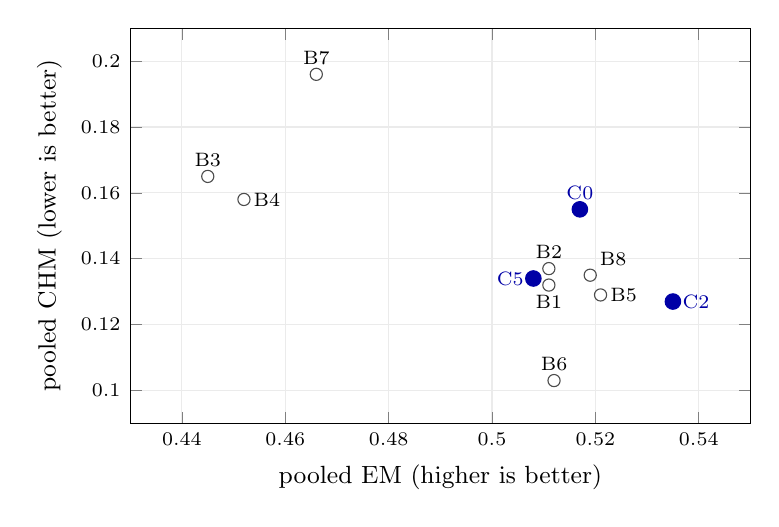
\begin{tikzpicture}
\begin{axis}[width=0.78\textwidth, height=6.6cm, xlabel={pooled EM (higher is better)}, ylabel={pooled CHM (lower is better)},
  xmin=0.43, xmax=0.55, ymin=0.09, ymax=0.21, font=\small, tick label style={font=\scriptsize}, grid=major, grid style={black!8}]
  \addplot[black!70, only marks, mark=o, mark size=2.2pt] coordinates {(0.511,0.132)};
  \node[font=\scriptsize, anchor=north] at (axis cs:0.511,0.132) {B1};
  \addplot[black!70, only marks, mark=o, mark size=2.2pt] coordinates {(0.511,0.137)};
  \node[font=\scriptsize, anchor=south] at (axis cs:0.511,0.137) {B2};
  \addplot[black!70, only marks, mark=o, mark size=2.2pt] coordinates {(0.445,0.165)};
  \node[font=\scriptsize, anchor=south] at (axis cs:0.445,0.165) {B3};
  \addplot[black!70, only marks, mark=o, mark size=2.2pt] coordinates {(0.452,0.158)};
  \node[font=\scriptsize, anchor=west] at (axis cs:0.452,0.158) {B4};
  \addplot[black!70, only marks, mark=o, mark size=2.2pt] coordinates {(0.521,0.129)};
  \node[font=\scriptsize, anchor=west] at (axis cs:0.521,0.129) {B5};
  \addplot[black!70, only marks, mark=o, mark size=2.2pt] coordinates {(0.512,0.103)};
  \node[font=\scriptsize, anchor=south] at (axis cs:0.512,0.103) {B6};
  \addplot[black!70, only marks, mark=o, mark size=2.2pt] coordinates {(0.466,0.196)};
  \node[font=\scriptsize, anchor=south] at (axis cs:0.466,0.196) {B7};
  \addplot[black!70, only marks, mark=o, mark size=2.2pt] coordinates {(0.519,0.135)};
  \node[font=\scriptsize, anchor=south west] at (axis cs:0.519,0.135) {B8};
  \addplot[blue!65!black, only marks, mark=*, mark size=2.8pt] coordinates {(0.517,0.155) (0.535,0.127) (0.508,0.134)};
  \node[font=\scriptsize, anchor=south, text=blue!65!black] at (axis cs:0.517,0.155) {C0};
  \node[font=\scriptsize, anchor=west, text=blue!65!black] at (axis cs:0.535,0.127) {C2};
  \node[font=\scriptsize, anchor=east, text=blue!65!black] at (axis cs:0.508,0.134) {C5};
\end{axis}
\end{tikzpicture}
\caption[CAEM and the baselines on EM and CHM.]{CAEM at C0, C2 and C5 (filled) and the eight baselines (open) on pooled EM and CHM in the model view (\Cref{tab:baseline-pooled}). The best systems sit at the lower right. The prompting baselines, B8 and CAEM form one cluster; the retrieval baselines sit apart at lower EM and higher CHM; the fine-tuned baseline B6 has the lowest CHM.}
\label{fig:baselines}
\end{figure}


% Auto-generated by scripts/paired_baseline_tests.py (final drafting pass 2026-10).
\begin{table}[!htbp]
\centering\small
\begin{tabular}{@{}lcccc@{}}
\toprule
 & \multicolumn{2}{c}{\textbf{CAEM C2}} & \multicolumn{2}{c}{\textbf{CAEM C5}} \\
\cmidrule(lr){2-3}\cmidrule(lr){4-5}
\textbf{Baseline} & \textbf{EM} & \textbf{CHM} & \textbf{EM} & \textbf{CHM} \\
\midrule
B1 zero-shot & 1 / 1 & 2 / 0 & 1 / 1 & 2 / 0 \\
B2 chain-of-thought & 1 / 1 & 2 / 0 & 1 / 1 & 2 / 0 \\
B3 RAG & 3 / 0 & 4 / 0 & 1 / 0 & 3 / 0 \\
B4 CoT + RAG & 3 / 0 & 4 / 0 & 1 / 0 & 3 / 0 \\
B5 five-shot CoT & 3 / 0 & 3 / 0 & 3 / 0 & 2 / 0 \\
B6 vanilla fine-tune & 1 / 0 & 3 / 1 & 1 / 0 & 2 / 1 \\
B7 FLARE & 1 / 1 & 5 / 0 & 0 / 1 & 5 / 0 \\
B8 semantic entropy & 1 / 0 & n/a & 1 / 0 & n/a \\
\midrule
Total & 14 / 3 of 40 & 23 / 1 of 35 & 9 / 3 of 40 & 19 / 1 of 35 \\
\bottomrule
\end{tabular}
\caption[Significant wins and defeats against each baseline.]{Significant wins / defeats of CAEM against each baseline over the five benchmarks (paired tests, Holm-corrected within each benchmark; \Cref{app:significance}). B8 has no valid CHM.}
\label{tab:sig-summary}
\end{table}


\textbf{Each baseline against its expectation:}
\begin{itemize}
    \item \textbf{Zero-shot (B1):}\label{sec:comp-zero-shot} the floor; the three-step comparison of \Cref{sec:headline-pooled} is built on it.
    \item \textbf{Chain of thought (B2):}\label{sec:comp-cot} expected to help on multi-step questions; instead it scored the same as B1 on pooled EM ($0.511$) with a slightly higher CHM ($0.137$), in line with Wei et al.~\cite{wei2022chain}, who find that the step-by-step cue helps little in models well below $100$ billion parameters, and Chung et al.~\cite{JMLR:v25:23-0870} for small instruction-tuned models. CAEM's zero-shot prompt already asks for reasoning before the answer, so B1 and B2 differ only in the added cue.
    \item \textbf{Retrieval (B3) and retrieval with chain of thought (B4):}\label{sec:comp-rag}\label{sec:comp-cot-rag} retrieving for every question lowered pooled EM ($0.445$ and $0.452$, against $0.511$ for B1) and raised CHM ($0.165$ and $0.158$), the strongest evidence in the panel that indiscriminate retrieval hurts on this backbone; CAEM's retrieval-utility classifier exists for this reason (\Cref{sec:ruc-ablation}).
    \item \textbf{Five-shot chain of thought (B5):}\label{sec:comp-fewshot} the strongest prompting baseline, with pooled EM $0.521$ and CHM $0.129$; its demonstrations help most on CommonsenseQA ($0.793$) and TruthfulQA ($0.347$, the best of any system), while on StrategyQA they hurt ($0.560$ against $0.643$ for B1).
    \item \textbf{Vanilla fine-tuning (B6):}\label{sec:comp-vanilla-ft} a full fine-tune of the backbone on the same training questions CAEM saw in each cycle ($2{,}000$ FEVER, $2{,}000$ TriviaQA and $700$ CommonsenseQA questions per cycle, five cycles, three epochs each), with the gold answer as the training target after CAEM's zero-shot prompt, and with no verifier filter, memory or retention guard. Unlike CAEM, it sees the correct answer for every training question, $23{,}500$ in all. It is the most accurate system on FEVER ($0.640$) and CommonsenseQA ($0.807$), the least accurate on TriviaQA ($0.290$) and TruthfulQA ($0.163$), and ends with pooled EM $0.512$, below CAEM at C2 and level with it at C5, and the lowest CHM ($0.103$). Its retention was not measured.
    \item \textbf{FLARE (B7):}\label{sec:comp-flare} retrieval triggered by low-confidence tokens did not avoid the cost of retrieval on this panel: pooled EM $0.466$ and the highest CHM ($0.196$).
    \item \textbf{Semantic-entropy abstention (B8):}\label{sec:comp-semantic-entropy} the closest comparator to CAEM's abstention. It withheld $75$ TriviaQA and $81$ TruthfulQA answers and almost none elsewhere, answering $89.5$ percent of all questions with an error among answered of $0.427$; its pooled EM is $0.519$ and its CHM $0.135$. Because semantic entropy measures disagreement across samples, it cannot flag a misconception the model holds consistently, as Farquhar et al.~\cite{farquhar2024semantic} note, and its TruthfulQA EM ($0.243$) stays at B1's level.
\end{itemize}
STaR and Self-RAG were not run: STaR's rationalisation step and binary filter differ too much from CAEM's verifier for a clean comparison, and Self-RAG's critic tokens are tied to a different model family.

\subsection{Retrieval-utility classifier ablation}
\label{sec:comp-ablations}
\label{sec:ruc-ablation}

The classifier is evaluated by comparing the main run with an earlier trajectory that ran without it, at cycle three, the last cycle both trajectories kept, with the composite fixed at the same cycle-three calibration so that the verifier signals are identical. The classifier-on run also carried some pipeline corrections (prompt fixes and minor bug fixes), so the comparison measures the classifier together with those corrections, not the classifier alone. Two acceptance gates were set in advance: (1) a pooled EM gain with no benchmark losing more than two points of EM, and (2) TruthfulQA EM reaching the B1 level. The B1 level was $0.433$ when the gate was set; under the final comparison protocol, with the judge reading only the final answer, it is $0.250$, and both runs are scored the same way.

% Generated by scripts/build_final_tables.py from outputs/analysis/chm_judged.json (label em_final); do not edit.
\begin{table}[!htbp]
\centering\small
\setlength{\tabcolsep}{2.5pt}
\renewcommand{\arraystretch}{1.15}
\begin{tabular}{@{}lrrrrrrrrr@{}}
\toprule
 & \multicolumn{3}{c}{\textbf{Exact match}} & \multicolumn{3}{c}{\textbf{CHM}} & \multicolumn{3}{c}{\textbf{Tier 3 share}} \\
\textbf{Benchmark} & \textbf{Off} & \textbf{On} & $\boldsymbol{\Delta}$\,(pp) & \textbf{Off} & \textbf{On} & $\boldsymbol{\Delta}$\,(\% rel) & \textbf{Off} & \textbf{On} & $\boldsymbol{\Delta}$\,(pp) \\
\midrule
\multicolumn{10}{@{}l}{\textit{Training panel}} \\
FEVER & $0.503$ & $0.503$ & $+0.0$ & $0.133$ & $0.137$ & $+2.5\%$ & $92.3\%$ & $70.7\%$ & $-21.7$ \\
TriviaQA & $0.437$ & $0.463$ & $+2.7$ & $0.141$ & $0.138$ & $-2.0\%$ & $95.7\%$ & $68.0\%$ & $-27.7$ \\
CommonsenseQA & $0.603$ & $0.743$ & $+14.0$ & $0.150$ & $0.098$ & $-34.4\%$ & $57.7\%$ & $20.3\%$ & $-37.3$ \\
\midrule
\multicolumn{10}{@{}l}{\textit{Transfer panel}} \\
StrategyQA & $0.617$ & $0.640$ & $+2.3$ & $0.136$ & $0.147$ & $+8.1\%$ & $100.0\%$ & $76.7\%$ & $-23.3$ \\
TruthfulQA & $0.177$ & $0.230$ & $+5.3$ & $0.160$ & $0.165$ & $+3.3\%$ & $99.0\%$ & $40.0\%$ & $-59.0$ \\
\midrule
\textbf{Pooled (all five)} & $0.467$ & $0.516$ & $+4.9$ & $0.144$ & $0.137$ & $-4.8\%$ & $88.9\%$ & $55.1\%$ & $-33.8$ \\
\bottomrule
\end{tabular}
\caption[Retrieval-utility classifier ablation at cycle three.]{CAEM without (Off) and with (On) the retrieval-utility classifier at cycle three, with the composite fixed at the cycle-three calibration: EM, CHM and retrieval share per benchmark.}
\label{tab:ruc-ablation}
\end{table}


\textbf{Gate 1 passes:} pooled EM rises from $0.467$ to $0.516$ ($+4.9$ points) with no benchmark losing EM; CommonsenseQA gains $14.0$ points, TruthfulQA $5.3$, TriviaQA $2.7$ and StrategyQA $2.3$, and FEVER is unchanged at $0.503$ (\Cref{tab:ruc-ablation}). Pooled CHM falls from $0.144$ to $0.137$, mostly on CommonsenseQA ($-34.4$ percent); on FEVER, StrategyQA and TruthfulQA it rises slightly ($+2.5$, $+8.1$ and $+3.3$ percent).

\textbf{Gate 2 fails, narrowly:} TruthfulQA EM rises from $0.177$ to $0.230$ but stays below B1's $0.250$, and its CHM rises slightly ($0.160$ to $0.165$, against $0.147$ for B1).

\textbf{Mechanism:} the retrieval share falls from $88.9$ to $55.1$ percent pooled, and on every benchmark, by $21.7$ points on FEVER, where retrieval genuinely helps, up to $59.0$ points on TruthfulQA ($99.0$ to $40.0$ percent), where it amplified misconceptions. Separating the classifier from the accompanying corrections would need a run with the corrections but without the classifier (\Cref{ch:conclusion}).

\section{Summary of Findings}
\label{sec:summary-findings}

\subsection{Headline outcome in one paragraph}
\label{sec:summary-headline}

Under a matched comparison protocol, CAEM performs at the level of strong prompting baselines, clearly better than retrieval baselines, and level on accuracy with a fine-tuned baseline that needs gold answers, but it does not reduce hallucination below the strong baselines. Pooled EM moves from $0.511$ (B1) to $0.517$ at C0, peaks at $0.535$ at C2 and ends at $0.508$ at C5; CHM moves from $0.132$ to $0.155$ at C0, where the system refuses too often, to $0.127$ at C2 and $0.134$ at C5. No difference between CAEM at C2 or C5 and B1 is significant on any benchmark. Self-improvement helps for one or two cycles and then erodes, and confident confabulation rises above B1's level as the gate becomes more permissive. What the architecture adds is selectivity: CAEM is wrong on $40.5$ percent of the questions it answers at C0 (B1: $48.9$ percent of all questions), and its status tag predicts correctness, with verified answers right $65$ to $75$ percent of the time. Its gains are concentrated where the verifier can check answers against retrieved passages, chiefly TriviaQA. The retrieval-utility classifier, with accompanying corrections, adds $4.9$ points of pooled EM.

\subsection{Hypothesis verdicts}
\label{sec:summary-hypotheses}

Each pre-specified hypothesis of \Cref{sec:hypotheses} is judged by its registered statistic, using only the three registered verdicts (\Cref{tab:hypothesis-verdicts}).

\begin{table}[!htbp]
\centering\small
\setlength{\tabcolsep}{4pt}
\begin{tabularx}{\textwidth}{@{}l>{\raggedright\arraybackslash}p{3.6cm}>{\raggedright\arraybackslash}p{2.2cm}>{\raggedright\arraybackslash}X@{}}
\toprule
\textbf{ID} & \textbf{Hypothesis (\Cref{sec:hypotheses})} & \textbf{Verdict} & \textbf{Deciding statistic and reading} \\
\midrule
H1 & Verifier balanced accuracy exceeds one half on the calibration-matched distribution at every cycle (\Cref{thm:bayes-purity} precondition). & \textbf{supported} & Pooled gate balanced accuracy on the calibration fold: $0.615$, $0.663$, $0.664$, $0.658$ at C1, C2, C3, C5 (C0 $0.753$, in-sample; \Cref{tab:gate-quality}). Weakest: CommonsenseQA $0.52$ to $0.55$; TriviaQA $0.500$ at C1, when no TriviaQA answer was stored. \\
H2 & Pool purity is non-decreasing across cycles whenever the precondition is satisfied (\Cref{thm:bayes-convergence}). & \textbf{unsupported} & Calibration-fold precision $0.780$ (C0, in-sample), $0.740$, $0.736$, $0.746$, $0.732$: it falls at C1, C2 and C5. The changes are within sampling noise and purity stays above the floor of \Cref{thm:purity} (\Cref{tab:pi-store-trajectory}). \\
H3 & Late-cycle pool-purity increments enter a bounded stationary band on the committed-cycle subsequence (\Cref{thm:convergence}). & \textbf{supported} & Precision within $0.732$ to $0.746$ at C1 to C5, a band of width $0.014$, about one standard error of a single reading; a convergence rate cannot be estimated in six cycles. \\
H4 & The composite hallucination metric at the realised cycle horizon approaches a parameter-bounded asymptote (\Cref{thm:asymptotic-elim}). & \textbf{partially supported} & CHM falls from $0.155$ to $0.131$ at C1 and stays between $0.127$ and $0.137$ afterwards ($0.134$ at C5), consistent with flattening; six cycles are too few to estimate the limit itself. \\
\bottomrule
\end{tabularx}
\caption[Hypothesis verdicts.]{Verdicts on the four pre-specified hypotheses.}
\label{tab:hypothesis-verdicts}
\end{table}

\FloatBarrier

\section{Discussion}
\label{sec:discussion}

\subsection{Headline interpretation}
\label{sec:disc-headline}

\textbf{What the matched comparison changed:} an earlier comparison gave the baselines a shorter prompt than CAEM's and scored some answer formats differently; under it, CAEM appeared to gain about three points of EM over B1 before any fine-tuning and to lead every baseline on CHM. Giving every system the same question message and the same scoring rule (\Cref{sec:setup-protocol}) removed most of that lead. On a three-billion-parameter generator, the prompt format alone moved the baselines' accuracy by several points, which is as large as the effects being measured; comparisons of small models are only as fair as their prompts.

\textbf{What carries the remaining gain:} the architecture's measurable contribution is selectivity rather than accuracy. The verifier's score, turned into a status tag and an abstention, lets CAEM tell the user which answers to trust: verified answers are right about two thirds of the time against about half for B1, and at C0 its answers are wrong less often than any baseline's. The self-improvement loop's main effect was behavioural: after one cycle the generator stopped refusing questions it could answer, which removed the cold-start over-refusal and gave the best EM and CHM of the run at C1 and C2. Its gains lasted one or two cycles, in line with Song et al.~\cite{song2024gap}, who find that self-improvement loops saturate within a few rounds.

\textbf{Why the theory does not promise more:} the purification results of \Cref{sec:theory} are about the stored pool, not the model. They held: the stored pool was purer than the generator's raw answers. Whether a model trained on a pool that is still about one-fifth wrong improves is a separate question, and Yi et al.~\cite{fu2025collapse} show that training filtered through a verifier converges to the verifier's own knowledge, mistakes included. The fall in zero-shot accuracy after C2 and the rise in confident confabulation are consistent with that, though the retraining on a cleaned pool that would show it was not run.

\textbf{Label efficiency:} CAEM is label-efficient, not label-free. A labelled calibration fold of $1{,}500$ questions fits the verifier's composite and thresholds, and each later cycle re-scores the same fold with the new adapter and refits; the $603$ cold-start answers were checked against gold labels once (\Cref{sec:memory-store}); every later training answer is labelled by the verifier alone, about $2{,}100$ gold labels in all. Vanilla fine-tuning (B6) needs a gold answer for each of its $23{,}500$ training questions. With that difference, CAEM reaches B6's pooled EM ($0.535$ at C2 and $0.508$ at C5, against $0.512$), while B6 reaches the lower CHM ($0.103$).

\textbf{TruthfulQA:} retrieval does not help on questions written to invite a misconception. At C0, retrieval-tier answers on TruthfulQA were right $21.4$ percent of the time against $29.9$ percent for zero-shot ones (\Cref{tab:per-tier-em}); the difference is partly selection, since the router sends the harder questions to retrieval, but it agrees with the classifier ablation, which gained $5.3$ points on TruthfulQA mainly by retrieving less (\Cref{sec:ruc-ablation}). With every system judged on its final answer, CAEM's TruthfulQA EM stays at B1's level throughout ($0.230$ to $0.277$ against $0.250$), and five-shot chain of thought is the most accurate system there ($0.347$).

\subsection{Where the verifier can check answers}
\label{sec:disc-verifier-scope}

The verifier's ability to separate correct from incorrect answers differs by benchmark. Its area under the ROC curve on the evaluation fold is $0.86$, $0.79$ and $0.75$ on TriviaQA at C0, C2 and C5, $0.64$ to $0.67$ on FEVER, and $0.51$ to $0.62$ on CommonsenseQA, StrategyQA and TruthfulQA. The difference follows from what the signals can see. The signals that carry information about correctness on this panel compare the answer with retrieved Wikipedia passages or, through the question-match score, with the question (\Cref{sec:verifier-qa-rel}); a trivia answer is either stated in a passage or not, while a commonsense choice, an implicit multi-step yes-or-no answer or a misconception is rarely settled by any single passage. The two internal signals do not make up for this: the token signal scores the whole response rather than the answer (\Cref{sec:verifier-internal}), and the dropout and chain signals measure agreement, which a consistently held mistake passes. CAEM's gains follow the same pattern. TriviaQA is where the architecture helps most (EM $0.463$ at C0 and $0.493$ at C2 against $0.430$ for B1), and the benchmarks where the verifier is close to chance are where CAEM is level with, or below, the strong baselines. A verifier that can judge commonsense and reasoning answers, or a system scoped to questions that can be checked against documents, are the two directions this points to (\Cref{ch:conclusion}).

\subsection{A side effect of self-improvement}
\label{sec:disc-phantom}

After the first fine-tune, almost every zero-shot answer began with a reference to ``the context'', although Tier 2 gives the generator no passages. The share of Tier 2 answers on the evaluation fold that mention a context in their first sentences was $3$ percent at C0 ($25$ of $731$), then $93$, $98$, $97$, $97$ and $99$ percent at C1 to C5 ($693$ of $747$ at C1, $746$ of $753$ at C5). The cause is the training data: the fine-tune learns from stored reasoning chains, and most of those were written under the retrieval prompt, where citing the context is correct. The answers can still be right, but each such answer cites a source that does not exist, which is a faithfulness error in its own right. Removing or rewriting context references in the training chains before fine-tuning would have prevented it; this preprocessing step was missed and is proposed in \Cref{ch:conclusion}.

\subsection{Threats to validity}
\label{sec:disc-threats}

\subsubsection{Single seed and single backbone}
\label{sec:disc-threat-seed}

All numbers come from one seed and one three-billion-parameter generator. Repeating the run with other seeds would turn the per-cycle readings into intervals, and repeating it with another generator of similar size would show whether the findings depend on this model.

\subsubsection{Benchmark coverage}
\label{sec:disc-threat-benchmark}

The panel covers short-answer factual and commonsense questions. Long-form generation, code, mathematics, dialogue and other languages are outside its scope (\Cref{sec:scope-research}), and the atomic-fact signal and the long-input judge, built for long answers, were not exercised.

\subsubsection{Calibration to evaluation gap}
\label{sec:disc-threat-gap}

The storage precision promised at the cut-point is measured on the calibration fold and holds on new data only as far as that data resembles it. On the training panel the gap stayed within about five points; on TruthfulQA it did not hold at all (\Cref{sec:check-purity}).

\subsubsection{Cycle budget}
\label{sec:disc-threat-cycles}

The run stopped after cycle five as planned (\Cref{sec:env-cycles}). Six cycles are too few to estimate convergence rates or long-run limits; that would need at least fifteen kept cycles.

\subsubsection{Storage-tail sample size}
\label{sec:disc-threat-n}

Per-benchmark numbers rest on few stored answers in places: at cycle zero the locked gate stored $93$ FEVER answers, $465$ CommonsenseQA answers and no TriviaQA answer on the validation fold, and Tier 1 gave only $7$ answers on the evaluation fold. Pooled readings are more reliable than per-benchmark ones.

\subsubsection{Retrieval-utility classifier mis-routing}
\label{sec:disc-threat-ruc}

The classifier's accuracy differs widely across benchmarks (AUROC $0.718$ on FEVER to $0.936$ on TriviaQA, \Cref{sec:ruc}), so questions unlike its training data may be routed the wrong way. It was not tested on a benchmark held out from its training data.

\subsubsection{Measuring hallucination with the system's own verifier}
\label{sec:disc-threat-verifier}

Two of the seven CHM subtypes depend on CAEM's own verifier: confident confabulation uses its stored score and false refusal uses its decision. The baselines have no verifier of their own, so their answers were scored with CAEM's verifier and the composite fixed at cycle three, and the verifier's decision on a baseline answer is not charged to the baseline (\Cref{sec:setup-protocol}). CHM differences are still partly measured with the instrument CAEM was built around. Two checks limit this concern:
\begin{itemize}
    \item \textbf{Without the two verifier-defined subtypes:} the other five use neither CAEM's composite score nor its decisions. Restricted to them, CAEM at C2 and C5 is lower than every baseline ($0.083$ pooled at both cycles, against $0.084$ for vanilla fine-tuning, the nearest, and $0.103$ for B1), and the paired test gives $28$ significant wins and $2$ defeats at C2 and $31$ wins and $3$ defeats at C5 out of $40$ contrasts. Part of this advantage is built in: the factual-fabrication flag checks answers against passages from the same retrieval that CAEM's retrieval tier writes its answers from.
    \item \textbf{Exact match and the delivered view's error among answered:} both are scored against gold labels and do not depend on the verifier's scores.
\end{itemize}

\subsection{Sensitivity analyses}
\label{sec:disc-sensitivity}

From the re-run sweep (\Cref{tab:sweep-variants}): moving the cut-point from $0.60$ to $0.65$ halves the number of stored answers ($560$ to $281$ on the calibration fold) and raises their precision ($0.780$ to $0.865$). Raising the regularisation strength $C$ from $0.01$ to $0.025$ or more stores far fewer answers on the validation fold ($313$ or fewer, against $558$) at a similar precision ($0.744$ to $0.772$, against $0.751$). Raising $\alpha_{\text{shrink}}$ stores more answers but separates correct from incorrect answers less well on the validation fold (pooled $d$ $0.85$ at $0$, $0.72$ at $0.6$, $0.66$ at $1$). Sensitivity to the safety floor and to the early-exit thresholds was not measured.

\subsection{Comparison to the strongest prior systems}
\label{sec:disc-prior}

\textbf{Conformal factuality:} Mohri and Hashimoto~\cite{mohri2024conformal} raise the correctness of GPT-4 answers from $78$ to $93$ percent on Natural Questions by removing low-scoring sub-claims at a split-conformal threshold, and Cherian et al.~\cite{cherian2024conformal} add conditional guarantees and a learned combination of claim scores. CAEM applies its gate when storing an answer rather than when showing it, keeps the gated answers for reuse, and combines its signals in the manner of Valentin et al.~\cite{valentin2024hallucination}; it also found that conformal guarantees broke under its calibration-to-evaluation shift (\Cref{sec:conformal-gate}).

\textbf{Verifier-filtered self-improvement:} STaR~\cite{NEURIPS2022_639a9a17} and V-STaR~\cite{hosseini2024vstar} train on their own correctness-filtered outputs, and Huang et al.~\cite{huang2025sharpening} analyse self-improvement as sharpening. CAEM differs in using an external multi-signal verifier and in keeping verified answers in memory; like those loops, its gains saturated quickly.

\textbf{Selective retrieval:} Adaptive-RAG of Jeong et al.~\cite{jeong2024adaptive}, the popularity-based routing of Mallen et al.~\cite{mallen2023whennot}, the self-knowledge routing of Wang et al.~\cite{wang2023skr} and the probing of Baek et al.~\cite{baek2025probing} all decide per question whether to retrieve. CAEM's classifier belongs to this line, and its ablation (\Cref{sec:ruc-ablation}) agrees with their finding that retrieving for every question leaves accuracy on the table.

\textbf{Retrieval and misconceptions:} on questions written to invite a familiar wrong answer, retrieved passages tend to share the question's framing rather than refute it, so the retrieval tier amplifies the misconception and the storage gate cannot recover what retrieval has already corrupted. This is why retrieval-tier answers on TruthfulQA are the least accurate of the panel (\Cref{sec:disc-headline}), and the case the classifier was built for.


\subsection{Limitations}
\label{sec:disc-limitations}

\begin{itemize}
    \item \textbf{Memory scale:} the memory reached $12{,}175$ entries, so its behaviour at the millions of entries of a deployment was not tested.
    \item \textbf{Pre-routing calibration:} the pre-routing temperature reached its upper bound at cycle zero ($T = 20.086$) on FEVER and TriviaQA, which flattened $\upre$ and left the safety override almost inactive (\Cref{sec:tier-safety}); the storage decision does not depend on this temperature.
    \item \textbf{Deferred-pool horizon:} only three reconsideration passes ran, so the long-run behaviour of the deferred buffer is not known.
    \item \textbf{Question-match signal:} the fourth signal family was meant to catch off-topic answers, but it scores the short answer string, which the cross-encoder cannot relate to the question; it acted as a correctness cue instead, and off-topic answers were not detected (\Cref{sec:verifier-qa-rel}).
    \item \textbf{Phantom context:} fine-tuning on retrieval-written chains taught the generator to cite a non-existent context (\Cref{sec:disc-phantom}).
    \item \textbf{Verifier scope:} the verifier separates correct from incorrect answers well only where retrieved passages can confirm an answer (TriviaQA), and is close to chance on commonsense, multi-step and misconception questions (\Cref{sec:disc-verifier-scope}).
    \item \textbf{Confident confabulation after self-improvement:} the verifier scores more of the fine-tuned generator's wrong answers highly than it did the base generator's ($0.305$ at C5 against $0.208$ for B1), so the gate's selectivity weakens as the generator it judges changes.
    \item \textbf{No repeated questions:} the evaluation uses fresh questions to measure learning, so the memory-direct path, built for repeated questions in deployment, and its cost saving were exercised only by the router probe; the gain in deployment depends on the share of repeats, which this study does not measure.
\end{itemize}

\paragraph{Limitations identified against the literature:} six further limitations follow from the cited literature.
\begin{itemize}
\item \textbf{Saturation and format learning:} Song et al.~\cite{song2024gap} report that verifier-filtered self-improvement saturates within two or three rounds and that part of the first-round gain at larger scales comes from better adherence to the answer format. The run is consistent with early saturation, and because the main metric is exact match, part of the early gain may be format learning; a flexible-match re-scoring would separate the two.
\item \textbf{Optimising toward the verifier:} Gulcehre et al.~\cite{gulcehre2023rest} find reward-model gains rising while human-judged quality peaks after the first round, and Yi et al.~\cite{fu2025collapse} show that verifier-filtered retraining converges to the verifier's own knowledge. Exact match against gold labels is independent of CAEM's verifier; CHM is not (\Cref{sec:disc-threat-verifier}).
\item \textbf{Systematic verifier errors:} agreement-based signals do not detect misconceptions the model holds consistently, as Farquhar et al.~\cite{farquhar2024semantic} warn, and repeated verification removes only independent errors (\Cref{cor:self-correction}); TruthfulQA's low stored precision is the realised case. The sample-agreement signal is an embedding cosine similarity, a family that Sinha~\cite{sinha2025semantic} shows can miss plausible hallucinations, although that evidence concerns similarity to a source rather than agreement across samples.
\item \textbf{Calibration-fold size:} Niculescu-Mizil and Caruana~\cite{niculescu2005predicting} find isotonic regression reliable only from about $1{,}000$ calibration points; CAEM fits per-benchmark curves on $500$ points, and the shrinkage toward the pooled fit limits but does not remove the resulting variance.
\item \textbf{Low chance floor:} Ho et al.~\cite{ho2023large} note that filtering on the final answer does not ensure correct reasoning, and Zelikman et al.~\cite{NEURIPS2022_639a9a17} that binary tasks yield many correct answers with poor rationales. StrategyQA and FEVER have chance levels of one half and one third, and FEVER answers enter the training pool.
\item \textbf{Adapter capacity and drift:} Biderman et al.~\cite{biderman2024lora} find that low-rank adaptation learns less of a new target than full fine-tuning and that its forgetting grows with training; the cycle-four rollback and the accuracy decline after cycle two are consistent with this, and the retention guard bounds the drift rather than preventing it.
\end{itemize}

\section{Chapter signpost}
\label{sec:ch5-signpost}

This chapter reported the main run, the cycle-zero choices behind it, the comparison with eight baselines and the classifier ablation, and judged the four hypotheses: H1 and H3 supported, H4 partially supported, H2 unsupported. \Cref{ch:conclusion} restates the contributions against these results and turns the limitations above into future work.
